\documentclass[a4paper,11pt,twoside]{article}
%\documentclass{book}

\usepackage[ngerman]{babel}
%\usepackage[top=3cm,bottom=3cm,left=3cm,right=3cm]{geometry} %NICHT IN KEMIE2


\usepackage{microtype} %schöneres typesetting  mit [stretch=10] für nur 1% anstelle von 2%
\usepackage{lmodern} %Latin Modern FONT
\usepackage{pifont} %schönere Font

\usepackage{chemfig}
\usepackage[version=4]{mhchem}
\usepackage{amsmath}
\usepackage{nicefrac}
\usepackage{amssymb}
%\usepackage{mathtools}

\usepackage{titlesec} %Um Section, etc bearbeiten zu können
\usepackage{fancyhdr}
\usepackage{setspace}
\usepackage{enumitem} %enumerate
\usepackage{arydshln} %für dashline
\usepackage{multicol}
\usepackage{lipsum}
\usepackage[labelfont=bf]{caption}

\usepackage[many]{tcolorbox}

%\usepackage{pgfornament} %Scheene Ornamente
\usepackage{witharrows} %Arrows in align-Umgebung
%\usepackage{awesomebox} %Notizboxen, etc
%\usepackage{textpos} %Für zum Beispiel vertikale Texte am Rand


%\usepackage{wrapfig} %Text um Bilder
%\usepackage{varwidth} % Alternative für engere minipage


\usepackage{hyperref}


\tcbuselibrary{theorems}

%\titlespacing*{\section}{0pt}{10mm}{3mm}
%\titlespacing*{\subsection}{0pt}{6mm}{3mm}
%\titlespacing*{\subsubsection}{0pt}{8mm}{3mm}


\renewcommand{\ttdefault}{lmtt} %Schriftart wird geändert zu Latin Modern Typewriter


\hypersetup{hidelinks,
			colorlinks=true,
			linkcolor=black,
			citecolor=miudiutex,
			urlcolor=miugray2
			}

\setlength\fboxsep{0pt}				
\setlength\columnsep{20pt}
\setlength{\parindent}{0pt}
\setcounter{section}{0}






%\definecolor{miudiutex}{HTML}{2f3d39}
\definecolor{miudiutex}{HTML}{1d2926}
\definecolor{miugray}{HTML}{b4cccf}
%\definecolor{miugray2}{HTML}{4d7365}
\definecolor{miugray2}{HTML}{6F8C81}
\definecolor{beige}{HTML}{F4F8D3}
\definecolor{white2}{HTML}{f5f7f8}
\definecolor{red}{HTML}{cf1f5c}
\definecolor{red2}{HTML}{9C191B}
\definecolor{green}{HTML}{00A36C}
\definecolor{delphinidin2}{HTML}{315794}
\definecolor{delphinidin}{HTML}{8B9EBA}
\definecolor{uniblau}{HTML}{004e9f}
\definecolor{unigelb}{HTML}{fcba00}
\definecolor{unigrau}{HTML}{909085}
\definecolor{pelargonidin}{HTML}{b33807}
\definecolor{pelargonidin2}{HTML}{FFDC96}
\definecolor{cyanidin}{HTML}{ba0746}
\definecolor{paeonidin}{HTML}{d15ca6}
\definecolor{petunidin}{HTML}{B88495}
\definecolor{petunitext}{HTML}{963354}
\definecolor{malvidin}{HTML}{8a2d8c}
\definecolor{mytheorembg}{HTML}{F2F2F9}
\definecolor{mytheoremfr}{HTML}{00007B}
\definecolor{uniblau2}{HTML}{27548A}
\definecolor{unigelb2}{HTML}{DDA853}
\definecolor{unidunkelblau2}{HTML}{183B4E}
\definecolor{unibeige}{HTML}{F5EEDC}


\tikzset{>=Latex}

\raggedcolumns %wichtig für Multicolumns
\color{miudiutex}



\usetikzlibrary{chains,
                positioning,
                shapes.multipart,
                }


\setchemfig
{%	
	bond offset=2pt,
	atom sep=15pt, 
	cram width=3pt,
	cram dash width=0.8pt,
	cram dash sep=1.2pt,
	double bond sep=2.5pt, 
	bond style={line width=1.1pt,cap=round},
	baseline=(current bounding box.center),
	bond join=true
}
\setcharge{extra sep=3pt}





%================================
% SYMBOLS
%================================

\newcommand{\RA}{$\rightarrow$~}
\newcommand{\RL}{$\rightleftharpoons$~}
\newcommand{\HARP}{\ding{226}~}
%$\xrightarrow{2}$ %Pfeil mit 2 drüber


%================================
% SHORT COMMANDS (BOXES ; ETC)
%================================


\newcommand{\info}[1]{\begin{note}{\color{miudiutex}#1}\end{note}}
\newcommand{\qsbig}[1]{\begin{qstion}{}{}\begin{center}
			#1 \end{center}\end{qstion}}
\newcommand{\notiz}[1]{\begin{notizz}{}{}\begin{center}
			{\color{miugray2!50!miudiutex}#1} \end{center}\end{notizz}}
\newcommand{\klausur}[1]{\begin{klausurinfo}{}{}\begin{center}
			#1 \end{center}\end{klausurinfo}}
\newcommand{\dfn}[1]{\begin{defin}{}{}\begin{center}
			#1 \end{center}\end{defin}}
\newcommand{\gesetz}[2]{\begin{gestex}{}{}\begin{center}
			#1 \end{center}\end{gestex}}
\newcommand{\gergesetz}[1]{\begin{gesgex}{}{}\begin{center}
			#1 \end{center}\end{gesgex}}
\newcommand{\klaausur}[1]{\begin{klausurinfo}[width=.77\linewidth]{}{}\begin{center}
			\footnotesize #1 \end{center}\end{klausurinfo}}
\newcommand{\winfo}[1]{\begin{wichtig}{}{} \begin{center}
#1 \end{center} \vspace*{0mm} \end{wichtig}}
\newcommand{\zit}[2]{\begin{zitat}{#1}{}\small #2 \end{zitat}}



\newcommand{\unten}{\end{center} \tcblower \begin{center}}


\newcommand*\circled[1]{\tikz[baseline=(char.base)]{
            \node[shape=circle,draw,inner sep=0.5pt,miudiutex] (char) {\tiny #1};}}
            
\newcommand{\miusquare}{{\color{miugray2!50}\scriptsize $\blacksquare$}~}
\newcommand{\miusquarp}{{\color{petunidin!50}\scriptsize $\blacktriangleright$}~}
\newcommand{\niu}{\item[\miusquare]}
\newcommand{\nip}{\item[\miusquarp]}
\newcommand{\mrk}[1]{{\color{petunitext!55!red}\textsc{#1}}}

%%%%% ABSAETZE

\newcommand{\pps}{\par \vspace*{1mm}}
\newcommand{\pp}{\par \vspace*{3mm}}
\newcommand{\ppbig}{\par \vspace*{8mm}}
\newcommand{\pphuge}{\par \vspace*{10mm}}



%================================
% HEADER & FOOTER FUER UNI
%================================
\newcommand{\miusfoot}{
\fancypagestyle{plain}{%
  \fancyhf{}%
  \renewcommand{\footrulewidth}{0.0mm}%
  \fancyfoot[L]{\hspace*{-3cm} {\color{miugray2}\textbf{\thepage}}}%
  \renewcommand{\headrulewidth}{0mm}%
} 
\pagestyle{plain}
}

\newcommand{\miushead}[2]{
\miusquare #1 - 4.Semester - ELW \hfill 
\includegraphics[width=60pt]{{F://LaTeX-Files/shiet/unibo}}
\par \vspace*{-3mm}
\hrulefill
\par \vspace*{1mm}
\par \vspace*{-4mm}
\normalsize	
	\begin{flushright}
	\textbf{\miusquare #2}\par \vspace*{1.5mm}
	\small	
	\textit{Letzte Überarbeitung:} \par 
	\footnotesize \today
	\end{flushright}
	\normalsize
\par \vspace*{-8mm}
}

\newcommand{\sidebar}{
\AddToHook{shipout/background}{
  \begin{tikzpicture}[remember picture,overlay, shift={(current page.south west)}]
   \path[fill=miugray2!15](0,0) rectangle (3.5cm,\paperheight);
%   \path[fill=miugray2!8](0,0) rectangle (3.5cm,\paperheight);
   \path[draw,miudiutex!50] (3.5,0) to (3.5,\paperheight);
%   \path[draw,miudiutex!50,dashed] (3.5,0) to (3.5,\paperheight);  
%   \node[opacity=0.8](a)at(12,10){\includegraphics[width=9cm]{F://LaTeX-Files/pngs/girl01}};
  \end{tikzpicture} 
}
}


\newcommand{\oddsidebar}{
\AddToHook{shipout/background}{
   \put(0in,-\paperheight){%
      \ifodd\value{page}\relax
           \begin{tikzpicture}[remember picture,overlay, shift={(current page.south west)}]
   \path[fill=miugray2!15](0,0) rectangle (3.5cm,\paperheight);
      \path[draw,miudiutex!50] (3.5,0) to (3.5,\paperheight);
  \end{tikzpicture}
      \else
           \begin{tikzpicture}[remember picture,overlay, shift={(current page.south east)}]
   \path[fill=miugray2!15](-3,0) rectangle (3cm,\paperheight);
%      \path[draw,miudiutex!50] (-3.5,0) to (-3.5,\paperheight);
  \end{tikzpicture}
      \fi
   }
}
}
%================================
% ENVIRONMENTS
%================================

\newenvironment{ctab}[2]{%
				\begin{spacing}{#1}
					\begin{center}
					\begin{tabular}{#2}}
					{\end{tabular}
					\end{center}
				\end{spacing}
				}


%================================
% Farbiger-Background-Box
%================================



\newcommand{\farbig}[1]{
\begin{tcolorbox}[%
				hbox,
				colback=miugray2!25,
				boxsep=-2pt,
				boxrule=0pt,
				arc=0pt,
				nobeforeafter,
				tcbox raise base,
				shrink tight,
				extrude by=1pt
				]
				{\color{miudiutex}{#1}}
\end{tcolorbox}~}

%================================
% SIMPLE SCHWARZER RAHMEN BOX
%================================


\newcommand{\boxfr}[1]{
	\begin{tcolorbox}[
	colframe=miugray2,
	colback=white!95!miugray2,
	boxrule = 0.5pt, 
%	toprule=0pt, bottomrule=0pt,rightrule=0pt,leftrule=0pt,
	boxsep=0pt,
	arc=4pt,
	drop shadow southeast,
	enhanced
	]
	\color{miudiutex}
	\begin{center}
	#1
	\end{center}
	\end{tcolorbox}
}

%================================
% Antwort-Box
%================================

\newcommand{\antwort}[1]{\par 
	\begin{tcolorbox}[
	colback=gray!15,
	breakable,
	enhanced,
	frame hidden,
	arc=5pt,
	boxrule = 2pt,
%	borderline west = {2pt}{0pt}{petunidin},
%	drop shadow=miugray2!30
	]
	\color{miudiutex}	#1
	\end{tcolorbox}
}

%================================
% Frame-IT
%================================

\newcommand{\frameit}[1]{\par 
	\begin{tcolorbox}[
	colback=gray!10,
	breakable,
	enhanced,
	frame hidden,
	arc=5pt,
	boxrule = 0pt,
	borderline west = {4pt}{0pt}{petunidin},
%	drop shadow=miugray2!30
	]
		#1
	\end{tcolorbox}
}



%================================
% Question BOX
%================================

\makeatletter
\newtcbtheorem{qstion}{Frage}{enhanced,
	breakable,
	colback=white,
	colframe=delphinidin!100,
%	capture=hbox,
	boxsep=-3pt,
	attach boxed title to top left={yshift*=-\tcboxedtitleheight},
	fonttitle=\bfseries,
%	title={#2},
	boxed title size=title,
	boxed title style={%
			sharp corners,
			rounded corners=northwest,
			colback=tcbcolframe,
			boxrule=0pt,
		},
	underlay boxed title={%
			\path[fill=tcbcolframe] (title.south west)--(title.south east)
			to[out=0, in=180] ([xshift=5mm]title.east)--
			(title.center-|frame.east)
			[rounded corners=\kvtcb@arc] |-
			(frame.north) -| cycle;
		},
	#1
}{def}
\makeatother



%================================
% SIMPLE Question BOX
%================================

\newcommand{\qssmall}{
\begin{tcolorbox}[hbox,colback=miugray2!55,boxsep=-4pt,boxrule=0pt,arc=2pt,nobeforeafter, tcbox raise base,shrink tight,extrude by=3pt]
\textbf{\color{white}{?}}
\end{tcolorbox}~~}

\newcommand{\folie}[1]{
\begin{tcolorbox}[%
				hbox,
				colback=miugray2!20,
				boxsep=2pt,
				boxrule=0.5pt,
				arc=2pt,
				nobeforeafter,
				tcbox raise base,
				shrink tight,
				extrude by=3pt]
				{\color{miudiutex}{Folie #1}}
\end{tcolorbox}~}


%================================
% NOTIZ BOX
%================================

\makeatletter
\newtcbtheorem{notizz}{Notiz}{enhanced,
	breakable,
	coltitle=white,
	colback=petunidin!10,
	colframe=petunidin!50,
	attach boxed title to top left={yshift*=-\tcboxedtitleheight},
	fonttitle=\bfseries,
%	title={#2},
	boxed title size=title,
	boxed title style={%
			sharp corners,
			rounded corners=northwest,
			colback=tcbcolframe,
			boxrule=0pt,
		},
	underlay boxed title={%
			\path[fill=tcbcolframe] (title.south west)--(title.south east)
			to[out=0, in=180] ([xshift=5mm]title.east)--
			(title.center-|frame.east)
			[rounded corners=\kvtcb@arc] |-
			(frame.north) -| cycle;
		},
		#1
}{def}
\makeatother



%================================
% Question BOX: Klausur
%================================

\makeatletter
\newtcbtheorem[no counter]{klausurinfo}{Klausurrelevant}{enhanced,
%	breakable,
	colback=miugray2!10,
	colframe=miugray2!75,
	attach boxed title to top left={yshift*=-\tcboxedtitleheight},
	fonttitle=\bfseries,
	title={#2},
	arc=4pt,
	boxrule=1pt,
	boxed title size=title,
	boxed title style={%
			sharp corners,
			rounded corners=northwest,
			colback=tcbcolframe,
			boxrule=0pt,
			arc=4pt,
		},
	underlay boxed title={%
			\path[fill=tcbcolframe] (title.south west)--(title.south east)
			to[out=0, in=180] ([xshift=5mm]title.east)--
			(title.center-|frame.east)
			[rounded corners=\kvtcb@arc] |-
			(frame.north) -| cycle;
		},
	#1
}{def}
\makeatother


%================================
% DEFINITION
%================================

\makeatletter
\newtcbtheorem[no counter]{defin}{Definition}{enhanced,
	breakable,
	colback=gray!10,
	colframe=gray,
	attach boxed title to top left={yshift*=-\tcboxedtitleheight},
	fonttitle=\bfseries,
	title={#2},
	arc=4pt,
	boxrule=1pt,
	fontlower=\footnotesize,
	collower=miugray2!50!miudiutex,
	boxed title size=title,
	boxed title style={%
			sharp corners,
			rounded corners=northwest,
			colback=tcbcolframe,
			boxrule=0pt,
			arc=4pt,
		},
	underlay boxed title={%
			\path[fill=tcbcolframe] (title.south west)--(title.south east)
			to[out=0, in=180] ([xshift=5mm]title.east)--
			(title.center-|frame.east)
			[rounded corners=\kvtcb@arc] |-
			(frame.north) -| cycle;
		},
	#1
}{def}
\makeatother

%================================
% Gesetzes-Text EU
%================================

\makeatletter
\newtcbtheorem[no counter]{gestex}{EU - Verordnung}{enhanced,
	breakable,
	colback=gray!10,
	colframe={gray!65!delphinidin},
	attach boxed title to top left={yshift*=-\tcboxedtitleheight},
	fonttitle=\bfseries,
	arc=4pt,
	boxsep=10pt,
	boxrule=1pt,
	fontlower=\footnotesize,
	collower=miugray2!50!miudiutex,
	boxed title size=title,
	overlay={%
			\node[xshift=-1cm,yshift=-1mm] at (frame.north east)
			{\includegraphics[width=8mm]{F://LaTeX-Files/shiet/eu}};
%			\node[draw,miugray2] at (frame.north) {{#2}}; 
			},%
	boxed title style={%
			sharp corners,
			rounded corners=northwest,
			colback=tcbcolframe,
			boxrule=0pt,
			arc=4pt,
		},
	underlay boxed title={%
			\path[fill=tcbcolframe] (title.south west)--(title.south east)
			to[out=0, in=180] ([xshift=5mm]title.east)--
			(title.center-|frame.east)
			[rounded corners=\kvtcb@arc] |-
			(frame.north) -| cycle;
		},
	#1
}{def}
\makeatother


%================================
% Gesetzes-Text Ger
%================================

\makeatletter
\newtcbtheorem[no counter]{gesgex}{Gesetzestext}{enhanced,
	breakable,
	colback=gray!10,
	colframe={gray!95!pelargonidin},
	attach boxed title to top left={yshift*=-\tcboxedtitleheight},
	fonttitle=\bfseries,
	title={#2},
	arc=4pt,
	boxrule=1pt,
	fontlower=\footnotesize,
	collower=miugray2!50!miudiutex,
	boxed title size=title,
	overlay={\node[xshift=-1cm,yshift=-3mm] at (frame.north east)
			{\includegraphics[width=8mm]{F://LaTeX-Files/shiet/ger}}; 
			},
	boxed title style={%
			sharp corners,
			rounded corners=northwest,
			colback=tcbcolframe,
			boxrule=0pt,
			arc=4pt,
		},
	underlay boxed title={%
			\path[fill=tcbcolframe] (title.south west)--(title.south east)
			to[out=0, in=180] ([xshift=5mm]title.east)--
			(title.center-|frame.east)
			[rounded corners=\kvtcb@arc] |-
			(frame.north) -| cycle;
		},
	#1
}{def}
\makeatother


%================================
% Question BOX: Wichtig
%================================

%\makeatletter
%\newtcbtheorem[no counter]{wichtig}{Wichtige Info}{enhanced,
%	breakable,
%	colback=pelargonidin2!80,
%	colframe=red2!100,
%	fonttitle=\bfseries,
%	title={#2},
%	leftrule=5mm,
%	boxed title size=title,
%	boxed title style={%
%			sharp corners,
%			rounded corners=northwest,
%			colback=tcbcolframe,
%			boxrule=0pt,
%		},
%	underlay boxed title={%
%			\path[fill=tcbcolframe] (title.south west)--(title.south east)
%			to[out=0, in=180] ([yshift=1mm,xshift=7mm]title.east)--
%			([yshift=1mm]title.center-|frame.east)
%			[rounded corners=\kvtcb@arc] |-
%			(frame.north) -| cycle;
%		},
%		watermark tikz={\draw[line width=2mm] circle (1.1cm)
%		node{\fontfamily{ptm}\fontseries{b}\fontsize{20mm}{20mm}\selectfont !};}],
%	attach boxed title to top left={xshift=5mm,yshift*=-\tcboxedtitleheight},
%	watermark zoom=0.65,
%	  underlay={%
%    \path[draw=none] (interior.south west) rectangle node[white]{\Huge \textbf{!}} ([xshift=-4mm]interior.north west);
%    },
%	#1
%}{def}
%\makeatother


\makeatletter
\newtcbtheorem[no counter]{wichtig}{Wichtige Info}{enhanced,
	breakable,
	colback=pelargonidin2!30,
	colframe=petunidin!100,
	fonttitle=\footnotesize\bfseries,
	title={#2},
	leftrule=4mm,
	boxed title size=title,
	boxed title style={%
			sharp corners,
			rounded corners=northeast,
			colback=tcbcolframe,
			boxrule=0pt,
		},
	underlay boxed title={%
			\path[fill=tcbcolframe] (title.south east)--(title.south west)
			to[out=180, in=0] ([yshift=2mm,xshift=-7mm]title.west)--
			([yshift=2mm]title.center-|frame.west)
			[rounded corners=\kvtcb@arc] |-
			(frame.north) -| cycle;
		},
		watermark tikz={\draw[line width=2mm] circle (1.1cm)
		node{\fontfamily{ptm}\fontseries{b}\fontsize{20mm}{20mm}\selectfont !};},
	attach boxed title to top right={yshift*=-\tcboxedtitleheight},
	watermark zoom=1.45,
	watermark opacity=0.35,
	  underlay={%
    \path[draw=none] (interior.south west) rectangle node[white]{\LARGE \textbf{!}} ([xshift=-4.3mm]interior.north west);
    },
    #1
}{def}
\makeatother





%================================
% ZITAT BOX
%================================

\tcbuselibrary{theorems,skins,hooks}
\newtcbtheorem{zitat}{Zitat}
{%
	enhanced,
	breakable,
	colback = gray!10!white,
	frame hidden,
	boxrule = 0sp,
	borderline west = {2pt}{0pt}{petunidin},
	sharp corners,
	detach title,
	before upper = \tcbtitle\par\smallskip,
	coltitle = gray!50!black,
	fonttitle = \bfseries\sffamily,
	description font = \mdseries,
	separator sign none,
	segmentation style={solid, gray!50!black},
}
{th}



%\usepackage[top=2cm,bottom=2cm,left=4cm,right=2cm,heightrounded,
%  marginparwidth=2.7cm, marginparsep=8mm]{geometry}
%  \usepackage[top=2cm,bottom=2cm,left=2cm,right=1cm,heightrounded,
%  marginparwidth=0.7cm, marginparsep=8mm]{geometry}
\usepackage[top=3cm,bottom=3cm,left=3cm,right=3cm,heightrounded]{geometry}
\usepackage{awesomebox}
\usepackage{marginnote}
%\setcounter{secnumdepth}{0}
\usepackage{letltxmacro}



\usepackage[strict]{changepage}
\usepackage{refcount}
\usepackage{titletoc}
\usepackage{tikzpagenodes}
\usetikzlibrary{calc}
\usetikzlibrary{patterns.meta}
\usetikzlibrary{calc,shapes.symbols,decorations.pathreplacing}



\colorlet{mycolor}{petunitext}
\colorlet{myc2}{miugray2!50!miudiutex}




\titlecontents{section}%
 	 	[10mm]
 	 	{\vspace{1.5\baselineskip} \large \sffamily \bfseries \color{myc2}}
 	 	{\hspace*{0em}\llap{\parbox[t]{40pt}{\hfill\color{mycolor}\thecontentspage}\hspace*{10pt}}}
 	 	{\thecontentspage}
 	 	{\sffamily \qquad }

\titlecontents{subsection}%
	 	 [12mm]
	  	{\vspace{.3\baselineskip}\normalsize \sffamily \color{myc2}}
	  	{\hspace*{0em}\llap{\parbox[t]{40pt}{\hfill\color{mycolor}\thecontentspage}\hspace*{10pt}}}
	  	{\thecontentspage}
 	 	{\sffamily\qquad}

\titlecontents{subsubsection}%
 	 	[14mm]
	 	{\vspace{.3\baselineskip}\normalsize \sffamily \color{myc2}}
 		{\hspace*{0em}\llap{\parbox[t]{40pt}{\hfill\color{mycolor}\thecontentspage}\hspace*{10pt}}}
	  	{\thecontentspage}
	  	{\sffamily\qquad}




\titlespacing*{\section}{0pt}{30mm}{6mm}
\titlespacing*{\subsection}{0pt}{18mm}{3mm}
\titlespacing{\subsection}{0pt}{12mm}{3mm}
\titlespacing*{\subsubsection}{0pt}{6mm}{3mm}
\titlespacing{\subsubsection}{0pt}{6mm}{2mm}
\titlespacing{\paragraph}{0pt}{6mm}{2mm}



\titleformat{\section}[hang]
		{\LARGE \sffamily \bfseries \color{miudiutex!80!miugray2}}
		{\thesection}
		{4mm}
		{}

\titleformat{\subsection}[hang]
		{\large \sffamily \bfseries \color{miudiutex!50!miugray2}}
		{\thesubsection}
		{4mm}
		{}

\titleformat{\subsubsection}[block]
		{\normalsize \bfseries \sffamily \color{miudiutex!50!miugray2}}%
		{\normalsize \color{petunitext} \thesubsubsection}
		{2mm}
		{}
		[ \color{miugray}{\titlerule[0.3pt]}]
		
\titleformat{\paragraph}
		{\large \bfseries \sffamily \color{petunitext}}
		{\footnotesize \theparagraph}
		{1mm}
		{}



\renewcommand*{\marginfont}{\scriptsize\color{miudiutex!30!miugray2}\sffamily}
\renewcommand{\textbf}[1]{\textsf{{\bfseries {#1}}}}
\renewcommand{\labelitemi}{\miusquare}
\renewcommand{\labelitemii}{\miusquarp}
\setitemize{itemsep=0pt,labelsep=5pt,leftmargin=20pt}
\LetLtxMacro\mn\marginnote






%\usepackage[fleqn]{amsmath}


%\usepackage{siunitx}
%\setlength{\parindent}{0pt}
%\setlength{\mathindent}{0cm}
\newcommand{\cm}{\text{cm}}
\newcommand{\m}{\text{m}}
\newcommand{\lite}{\text{l}}
\newcommand{\kg}{\text{kg}}
\newcommand{\km}{\text{km}}
\newcommand{\h}{\text{h}}
\newcommand{\s}{\text{s}}
\newcommand{\tonne}{\text{t}}

\newcommand\ddfrac[2]{\frac{\displaystyle #1}{\displaystyle #2}}
\newgeometry{top=2cm,bottom=2cm,left=2cm,right=1cm,heightrounded, marginparwidth=0.7cm, marginparsep=8mm}

\pagestyle{empty}



\raggedbottom



















\begin{document}



\AddToHookNext{shipout/background}{
\begin{tikzpicture}[remember picture, overlay]
   \draw[miugray2!75,fill=miugray2!75, shift={(current page.north west)}] (-3,-2) rectangle (15,-5);
%   \draw[petunitext,fill=petunitext, shift={(current page.north west)}] (15.2,-2) rectangle (15.4,-5);
	\node[rotate=0,white!35, align=left,scale=1.8] (a)at(8.5,-4){\bfseries \sffamily  Prozessbezogene \\ \LARGE \bfseries \sffamily Lebensmitteltechnologie};
\end{tikzpicture}
}
\par \vspace*{2.5cm}
\hspace*{7cm} {\large \color{miugray2!50!miudiutex} SoSe 2025 - Dr. Helene Loos}



\par \vspace*{3cm}
\renewcommand{\contentsname}{
\Huge
\color{petunitext}\textbf{I} \color{myc2}\textbf{Fragebogen - Übersicht}
\normalsize
%\par \vspace*{-4mm}
%\hrulefill
}
{
  \hypersetup{linkcolor=myc2}
\tableofcontents
}

\vfill











\pagebreak
\AddToHook{shipout/background}{
\begin{tikzpicture}[remember picture, overlay]
\checkoddpage
\ifoddpage
   \draw[petunitext,fill=petunitext, shift={(current page.south west)},yshift=2cm] (0,0)rectangle (1,1) node[below,xshift=-0.5cm,yshift=-2mm] {\color{white} \LARGE \bfseries \sffamily \thepage} ;
%   \draw[miugray2,fill=miugray2, shift={(current page.north east)},yshift=-1cm] (0,0)rectangle (-1.7,-0.7) node[above,xshift=0.9cm,yshift=0mm] {\color{white} \large \bfseries \sffamily Excerpt} ;
   \draw[miugray2!75,line width=4pt, shift={(current page.north west)}] (4.1,0) to (4.1,-1.2);
\else
   \draw[petunitext,fill=petunitext, shift={(current page.south east)},yshift=2cm] (0,0)rectangle (-1,-1) node[below,xshift=0.5cm,yshift=8mm] {\color{white} \LARGE \bfseries \sffamily \thepage} ;
%   \draw[miugray2,fill=miugray2, shift={(current page.north east)},yshift=-1cm] (0,0)rectangle (-1.7,-0.7) node[above,xshift=0.9cm,yshift=0mm] {\color{white} \large \bfseries \sffamily Excerpt} ;
   \draw[miugray2!25,fill=miugray2!25, shift={(current page.north east)}] (-0.5,0) rectangle (-1.5,-4);
	\node[rotate=90,white!35] (a)at(20,-2.75){\LARGE \bfseries \sffamily PLMT};
\fi
\end{tikzpicture}
}

\section{Strömungslehre \& Rheologie}

\begin{multicols}{2}

\begin{enumerate}[label=\textbf{\arabic*}]
\item Was sind Fluide?
\antwort{
Als Fluid werden Substanzen bezeichnet, die sich unter dem Einfluss von \textbf{Scherkräften} kontinuierlich \textbf{verformen}, d. h. sie fließen. \pp
Sowohl Gase als auch Flüssigkeiten werden als Fluid bezeichnet.
}
\item Inwiefern unterscheiden sich Gase und Flüssigkeiten hinsichtlich ihrer Kompressibilität?
\antwort{Gase sind kompressibel, Flüssigkeiten nicht. \pp
\textit{Wobei sich auch Flüssigkeiten in gewissem Maße kompressieren lassen. Und strömende Gase beispielsweise bei geringer Geschwindigkeit und konstanter Temperatur als nahezu inkompressibel gelten.}}
\item Was ist die Hauptaussage der Kontinuitätsgleichung?
\antwort{Die Strömungsgeschwindigkeit in einem Körper bei konstantem Druck ist proportional abhängig von der Fläche.}
\item Was versteht man unter idealen und realen Fluiden?
\antwort{Bei idealen Fluiden werden Eigenschaften wie Kompressibilität oder Viskosität vernachlässigt, während sie bei realen Fluiden existieren.}
\item Was besagt das Gesetz von Bernoulli? Inwiefern ist die Gültigkeit des Gesetzes von Bernoulli
beschränkt?
\antwort{Summe aus Druckenergie, kinetischer und potentieller Energie bleibt immer konstant.
\begin{align*}
v + \rho g h + \frac{1}{2}\rho v^2 = konst.
\end{align*}
\footnotesize
\textit{Gilt nur für stationäre und verlustfreie Strömungen und inkompressible Fluide.}
}
\item Was besagt die Gleichung von Torricelli? 
\antwort{
Die Austrittsgeschwindigkeit eines Wasserstrahls aus der Öffnung hängt nur vom Füllstand, nicht von seiner Form oder der Größe der Austrittsöffnung ab.
\begin{align*}
v = \sqrt{2gh}
\end{align*}
}
\item Inwiefern ist die Gültigkeit der Gleichung von Torricelli beschränkt?
\antwort{Die Gleichung von Toricelli gilt nur für bestimmte Bedingungen. So gilt wieder, dass die Strömung \textbf{verlustfrei} sein muss und das Fluid \textbf{inkompressibel}. Desweiteren werden eckige oder besonders große Ausflussöffnungen nicht berücksichtigt.}


\pagebreak
\item Was versteht man unter der dynamischen und kinematischen Viskosität einer Flüssigkeit?
\antwort{
Die Unterschiede lassen sich am ehesten mit denen dazugehörigen Formeln beschreiben:\par 
Für die dynamische Viskosität $\eta$ [$\frac{kg}{m \cdot s}$] gilt:
\begin{align*}
\eta = \frac{\tau}{D}
\end{align*}
Für die kinematische Viskosität $\nu$ [$\frac{m}{s^2}$] gilt:
\begin{align*}
\nu = \frac{\eta}{\rho}
\end{align*}
}
\item Was versteht man unter Schubspannung und Schergeschwindigkeit (= Scherrate)?
\antwort{
Die \textbf{Schubspannung} bezeichnet die Kraft, die auf eine Fläche $A$ wirkt, wenn eine andere Kraft parallel zur Scherbewegung in die entgegengesetzte Richtung wirkt (Welche Kraft aufgewendet wird, damit das Fluid fließt). \pp
Die \textbf{Schergeschwindigkeit} beschreibt die Veränderung der Flussgeschwindigkeit eines Fluides aufgrund einer Scherung dieses Fluids (Wie schnell das Fluid fließt). \par 
}
%\pagebreak
\item Was versteht man unter einer Newton’schen Flüssigkeit?
\antwort{Bei einem Newtonschen Fluid verhält sich die Schergeschwindigkeit proportional zur Scherspannung}
\columnbreak
\item Was versteht man unter einer laminaren und turbulenten Strömung? Worin unterscheiden sich
laminare und turbulente Rohrströmungen und was sind die Konsequenzen in der Praxis?
\antwort{
Bei einer \textbf{laminaren Strömung} haben wir glatte, parallele Stromlinien und geringe Reibungsverluste. \par 
Bei einer \textbf{turbulenten Strömung} gibt es Verwirbelungen und höhere Reibungsverluste. 
\pp
Ob eine Strömung laminar oder turbulent ist hängt unter anderem von der Reynoldszahl ab. (Re$_{krit}$ $\approx$ 2300) \par 
In der Praxis bedeuten turbulente Rohrströmungen oft das Auftreten von Kavitationen, die das Rohr beschädigen können. 
}
\item Ist für den Wirbelwiderstand eines angeströmten Körpers hauptsächlich die Vorder- oder die Rückseite des Körpers von Bedeutung?
\antwort{Die Rückseite, da dort die Strömung abreißt und ein turbulenter Nachlauf entsteht.}
\item Ist das parabelförmige Geschwindigkeitsprofil der laminaren Rohrströmung bereits in der
Anlaufströmung ausgebildet?
\antwort{ Das parabelförmige Geschwindigkeitsprofil ist nicht von Anfang an komplett ausgebildet, sondern baut sich mit fortschreitender Anlaufströmung immer weiter aus.}










%\pagebreak
\item Wofür verwendet man das Moody-Diagramm und wie sieht es aus?
\antwort{ Das Moody-Diagramm zeigt im logarithmischen Maßstab den Zusammenhang zwischen Reibungskoeffizient, Reynoldszahl und Relativer Rauheit.
% \par
%So können etwaige Ergebnisse direkt abgelesen werden ohne sie berechnen zu müssen.
}
\pagebreak
\item Was versteht man unter den Begriffen Rohrleitungskennlinie und Pumpenkennlinie?
\antwort{
\textbf{Rohrleitungskennlinie} (auch Anlagenkennlinie): \par 
Beschreibt, das mit zunehmendem Volumenstrom der aufzuwendende Druck exponentiell ansteigt.
Dies lässt sich auch anhand der Basisgleichung für den Druckverlust veranschaulichen
\begin{align*}
\Delta p = \frac{\lambda \cdot l \cdot \rho}{d_i \cdot 2} \cdot v^2
\end{align*}
\textbf{Pumpenkennlinie:} \par 
Beschreibt, dass die Pumpe mit ihrer vorhandenen Leistung bei abnehmender Förderhöhe (bzw. $\Delta P_{ges}$) einen höheren Volumenstrom leisten kann.\pp
Herleitung der Pumpenkennlinie über die Gleichung für die Leistung einer Pumpe:
\begin{align*}
P &= \rho \cdot g \cdot h \cdot \dot{V} \\
h &= \frac{P}{\rho \cdot g \cdot \dot{V}}
\end{align*}
Diese Gleichung veranschaulicht nochmal, dass mit steigendem Volumenstrom die Förderhöhe sinken muss.
}
\item Anhand welcher Kriterien kann man Pumpen einteilen?
\antwort{
Wir unterscheiden vorallem zwischen: \par
\begin{itemize}
\item \textbf{volumetrisch} wirkenden Pumpen (Verdrängerpumpen)
\item \textbf{dynamisch} wirkenden Pumpen (Beschleunigung des zu pumpenden Fluids)

\end{itemize}
}

\columnbreak
\item Was versteht man unter Kavitation? Ist Kavitation erwünscht oder unerwünscht?
\antwort{
\textbf{Kavitation} kann als Folge von Druckschwankungen, welche durch unterschiedliche
Strömungsgeschwindigkeiten entstehen, auftreten. \pp
 Dabei bilden sich in der Flüssigkeit \textbf{Hohlräume}, die kurz darauf \textbf{implodieren}. Diese Implosionen \textbf{können Rohrwände beschädigen} und sind daher \textbf{unerwünscht}.
}




%\pagebreak
\item Welche Anforderungen gelten für den Transport von Lebensmitteln? Welche apparative Ausstattung wird für Transportvorgänge verwendet?
\antwort{
\begin{itemize}
\item \textbf{Schonende Förderung} \RA scherkraftarm, keine mechanischen Verletzungen
\item gute \textbf{Reinigungsmöglichkeiten}
\item \textbf{Material} geeignet \RA korosionsbeständig, keine Migration oder Abrieb
\item Gleichmäßiger, pulsationsfreier \textbf{Transport}
\end{itemize}
}
\pagebreak
\item Mit welchen Messgeräten kann man das rheologische Verhalten von Lebensmitteln bestimmen?
\antwort{
\textbf{Rheometer:}
\par
\begin{itemize}
\item Auslaufbecher
\item Kugelfall-Viskosimeter
\item Kapillar-Viskosimeter
\item Rotations-Viskosimeter
\end{itemize}
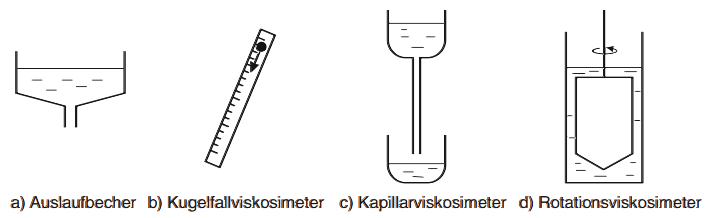
\includegraphics[width=\columnwidth]{misc/rheo}
\pp
\textbf{Rotationsviskosimeter} werden üblicherweise \textbf{bevorzugt}, da in ihnen eine exakt
definierte Strömung vorliegt und die Resultate besser interpretiert werden können.
Man unterscheidet hierbei Messsysteme mit zylindrischen, kegelförmigen, flachen und besonders geformten Drehkörpern.
}
\item Was versteht man unter Thixotropie?
\antwort{
Viskositätsabnahme eines Fluids über die Zeit einer konstanten Scherbeanspruchung. Danach vollständige (!) Regeneration.
}


%\columnbreak

\item Was versteht man unter pseudoplastischem und dilatantem rheologischen Verhalten und was sind
mögliche Gründe für ein solches Verhalten?


\antwort{
Am besten lassen sich die Begriffe über ihre Synonyme \textbf{scherverdickend (dilatant)} und \textbf{scherverdünnend (pseudoplastisch)} erklären. 
\pp 
So nimmt bei \textbf{scherverdickenden Flüssigkeiten} die Viskosität bei Scherbelastung zu (Oobleck \RA Stärke-Teilchen verkannten in einander). 
\pp
Bei \textbf{scherverdünnenden Flüssigkeiten} nimmt die Viskosität bei Scherbelastung ab (Proteine die vorher vernetzt waren, richten sich nun in Scherrichtung aus und führen zur Viskositätsabnahme).
}
\item Welche Auswirkungen hat viskoelastisches Verhalten bei lebensmitteltechnologischen Prozessen? 


\antwort{
\textbf{Pumpen} \par
Viskoelastische Flüssigkeiten können nicht-newtonsches Verhalten zeigen, was die Fließgeschwindigkeit und den Druckverlust in Rohrleitungen und Pumpen beeinflusst.
\pp
\textbf{Rühren} \par 
Polymerfäden kriechen an Rührwerkswelle empor, da sie unmittelbar an der Welle durch
Scherbeanspruchung gestreckt werden (Weissenberg-Effekt).
\pp
\textbf{Extrusion} \par 
bei Extrusion durch eine Düse weitet sich der Strang auf, d.h. er wird im Durchmesser deutlich größer als die Düsenöffnung (z.B. bei Polymerlösungen und –schmelzen).
In der Düse werden die Polymerketten gestreckt, nach der Düse kehren sie in geknäuelte ungeordnete Form zurück.
}
\end{enumerate}
\vfill 
%\begin{align*}
%\dot{Q} = \frac{d Q}{d t}
%\end{align*}





\end{multicols}










\pagebreak



\section{Wärme}
\begin{multicols}{2}
\begin{enumerate}[label=\textbf{\arabic*}]
\item Was versteht man unter der spezifischen Wärmekapazität bzw. wie kann man diese anschaulich
erklären? Wovon kann die spezifische Wärmekapazität eines Stoffes abhängen?
\antwort{
Die spezifische Wärmekapazität ist ein Maß für diejenige Energie, die man benötigt, um 
\textbf{1 kg eines Stoffes um 1 K (bzw. 1°C) zu erwärmen.} \ppbig
Sie hängt unter anderem von \textbf{intramolekularen Kräften} ab, aber auch Faktoren wie zum Beispiel die \textbf{Molmasse} beeinflussen die Wärmekapazität. 
}

\item Wie ist eine Kalorie definiert?
\antwort{ Eine Kalorie ist die Energie die benötigt wird um 1 g Wasser um 1 K zu erwärmen. \pp
\textbf{1 Kalorie = 4,18 Joule.} \pp Gängig ist auch die Bezeichnung Kilokalorie \RA 1kg Wasser um 1 K erwärmen benötigt 4180 Joule}









\item Aus welchen Gründen ist Wasser ein beliebter Stoff als Medium für Kühl- oder Heizprozesse?
\antwort{
Wasser hat eine \textbf{hohe Wärmekapazität} und zusätzlich eine \textbf{gute Wärmeleitfähigkeit} (Wärme kann gut abtransportiert werden. Desweiteren ist Wasser günstig und umweltverträglich.)
}
\item Bei welchen Prozessen der Lebensmittelverarbeitung ist die Übertragung von Wärme erforderlich?
\antwort{
\par \vspace*{-4mm}
\begin{multicols}{2}

\textbf{Zubereitung:}
\begin{itemize}
\item Kochen
\item Braten
\item Backen
\end{itemize}

\columnbreak

\textbf{Haltbarmachen:}
\begin{itemize}
\item Sterilisation
\item Pasteurisieren
\item Trocknen
\item Kühlen
\item Einfrieren
\end{itemize}

\end{multicols}
}
\columnbreak
\item Welche Arten der Wärmeübertragung unterscheidet man und was sind die zugrundeliegenden
Prinzipien? Für welche Arten der Wärmeübertragung benötigt man ein stoffliches Trägermedium?
\antwort{
\begin{itemize}
\item Wärmeleitung (Konduktion)
\item Wärmestrahlung (Radiation)
\item Wärmekonvektion

\end{itemize}
\par 
Die Wärmestrahlung benötigt, im Gegensatz zu den anderen beiden Wärme\-über\-tra\-gungs\-arten, kein Träger\-medium.
}
\item Welche Rolle spielt der Aggregatzustand von Stoffen für Wärmeübertragungsprozesse (Gase,
Flüssigkeiten, Feststoffe)? Was ist der Unterschied zwischen Wärme und Temperatur?
\antwort{
\textbf{Feststoffe} leiten Wärme circa 10 bis 100 mal \textbf{besser} als Fluide (besonders elektrische Leiter). Die Wärmeübertragung durch \textbf{Fluide} kann über \textbf{Konvektion} effizienter gemacht werden. 
\pp
\textbf{Wärme} ist die Energie, die übertragen wird, während \textbf{Temperatur} ein Maß für die Energie der Teilchen ist. 
}
\item Wie kann man elektromagnetische Wellen einteilen?
\antwort{
Hauptsächlich nach ihrer \textbf{Wellenlänge}. Beispiele: Gamma-, Röntgen-, UV-, Infrarotstrahlung usw.
}
\item Was versteht man unter dem Begriff „Wärmestrahlung“?
\antwort{
\textbf{Wärmestrahlung} ist die Strahlung, die ein Körper abgibt, wenn er sich über dem absoluten Nullpunkt befindet. \par Oft wird im Alltag fälschlicherweise nur die sichtbare glühend heiße Form als Wärmestrahlung bezeichnet.
}








\pagebreak

\item Was passiert, wenn Infrarotstrahlung auf einen Körper trifft? Was versteht man in dieser Hinsicht unter einem schwarzen, einem weißen, einem diathermanen, einem grauen und einem farbigen
Körper?
\antwort{
Infrarotstrahlung kann absorbiert, reflektiert oder durchgelassen (transmittiert) werden. 
\begin{itemize}
\item \textbf{Schwarzer Körper:} Absorbiert 100\% der Strahlung.
\item \textbf{Weißer Körper:} Reflektiert 100\% der Strahlung.
\item \textbf{Diathermer Körper:} Transmittiert Strahlung.
\item \textbf{Grauer Körper:} Absorbiert einen Teil der Strahlung; Reflektiert einen Teil der Strahlung. Wellenunabhängig.
\item \textbf{Farbiger Körper:} Absorbiert einen Teil der Strahlung; Reflektiert einen Teil der Strahlung. Wellenabhängig.

\end{itemize}

}

\item Was besagt das erste Kirchhoff’sche Gesetz?
\antwort{
Strahlungsabsorption und -emission entsprechen bei gegebener Wellenlänge einander: 
\par  \boxfr{Ein Körper, der gut absorbiert, strahlt auch gut.}
\pp
Die Strahlungsleistung verteilt sich allerdings nicht über alle Wellenlängen gleichmäßig, sondern wird durch das Plancksche Strahlungsgesetz bestimmt. Die Bestimmung des Maximums erfolgt über das \textbf{Wiensche Verschiebungsgesetz}. 

}
\item Was besagt das Wien’sche Verschiebungsgesetz?
\antwort{
Das \textbf{Wiensche Verschiebungsgesetz} besagt, dass die Wellenlänge, bei der ein Körper die meisten elektromagnetischen Wellen emittiert, mit zunehmender Temperatur des Körpers abnimmt. \pp
Das heißt: \textbf{Je heißer} ein Körper ist, \textbf{desto kürzer} ist die Wellenlänge der Strahlung, die er emittiert. 

}
\columnbreak
\item Was besagt das Stefan-Boltzmann’sche Gesetz?
\antwort{
Das Stefan-Boltzmann-Gesetz gibt die thermisch abgestrahlte Leistung eines idealen Schwarzen Körpers in Abhängigkeit von seiner Temperatur an.
\begin{align*}
P = \sigma \cdot A \cdot T^4
\end{align*}
}


\item Was besagt das erste Fourier’sche Gesetz?
\antwort{
Das Fouriersche Gesetz beschreibt den Wärmestrom der durch Wärmeleitung durch ein Material tritt. Dabei ist der Wärmefluss proportional zum Temperaturgradienten.
\begin{align*}
\dot{Q} = \lambda \cdot A \cdot \frac{T_{Warm}-T_{Kalt}}{d}
\end{align*}
Wobei $\lambda$ die Wärmeleitfähigkeit darstellt mit
\begin{align*}
\lambda = \frac{\text{W}}{\text{m} \cdot \text{K}}
\end{align*}
}




%\pagebreak

\item Was versteht man unter der Wärmeleitfähigkeit bzw. wie kann man diese anschaulich erklären?
\antwort{
Die Wärmeleitfähigkeit ist eine \textbf{Materialkonstante}. Sie beschreibt wie gut ein Material Wärme leiten kann. \textit{Wie viel Energie kann pro Meter und Kelvin übertragen werden?}
}
\item Was besagt das zweite Fourier’sche Gesetz?
\antwort{
Nach dem zweiten Hauptsatz der Thermodynamik:
\begin{center}
\textit{'Wärme wird immer von einem Gebiet mit höherer Temperatur zu einem Gebiet mit
niedrigerer Temperatur übertragen.'}
\end{center}

\textbf{Zweites Fouriersche Gesetz} (Fourier'sche Differentialgleichung): Sie beschreibt die räumliche Ausbreitung der Temperatur über die Zeit und ist definiert als:
\begin{align*}
\frac{\partial T}{\partial t} = \frac{\lambda}{\rho \cdot c_p} = \alpha \cdot \frac{d^2T}{dx^2}
\end{align*}
\href{https://www.tec-science.com/de/thermodynamik-waermelehre/waerme/warmeleitungsgleichung-diffusionsgleichung/}{\textbf{\RA Hier ausführlicher erklärt $\leftarrow$}}
}



\pagebreak
\item Wie kann man die Temperaturleitzahl interpretieren?
\antwort{
Die Temperaturleitzahl ist das Ergebnis des zweiten Fourierschen Gesetz. Sie beschreibt die \textbf{räumliche und zeitliche Ausbreitung der Temperatur} und beschreibt in welcher Zeit sich  die Temperatur im Material angleicht.
}




%\pagebreak

\item Wie beschreibt das Schichtenmodell den Wärmeübergang durch Konvektion?
\antwort{
An der Grenzfläche bildet sich eine ruhende (hydrodynamische) Grenzschicht, in der Wärme nur durch 
Leitung übertragen wird. 

		\begin{center}
Konvektion von laminarer gegenüber turbulenter Strömung
\begin{tikzpicture}
\node(a)at(0,0){
\begin{tikzpicture}

\draw[fill=miugray2!15,  postaction={pattern color=miugray2!50,pattern={Dots[angle=-45, distance=2mm,radius=0.7pt]}}] (-0.2,0) rectangle (0.3cm,2cm);
\draw[->,miugray2] (0.6,0) to (0.6,0.3);
\draw[->,miugray2] (1,0) to (1,0.7);
\draw[->,miugray2] (1.4,0) to (1.4,1);
\draw[->,miugray2] (1.8,0) to (1.8,1.2);
\draw[-,dashed,miugray2] (0.3,0) to [bend left=25] (1.8,1.2);
\node[miugray2,align=left,anchor=west,scale=0.6](1)at(2,0.5){Geschwindigkeitsprofil \\ laminare Strömung};
\draw[petunitext,-] (0.3,0.5) node[left,xshift=1mm] {$T_1$} to (1.8,1.6) node[right] {$T_2$};
\draw[->,delphinidin] (1.8,1.8) to node [above] {$\dot{Q}$} (-0.5,1.8)  ;
\draw[->,black!60] (1.8,-0.1) to node [below] {x} (-0.5,-0.1)  ;
\end{tikzpicture}
};
\node(b)at(0,-3.5){
\begin{tikzpicture}

\draw[fill=miugray2!15,  postaction={pattern color=miugray2!50,pattern={Dots[angle=-45, distance=2mm,radius=0.7pt]}}] (-0.2,0) rectangle (0.3cm,2cm);
\draw[->,miugray2] (0.6,0) to (0.6,0.3);
\draw[->,miugray2] (1,0) to (1,0.4);
\draw[->,miugray2] (1.4,0) to (1.4,0.4);
\draw[->,miugray2] (1.8,0) to (1.8,0.3);
\draw[-,dashed,miugray2] (0.3,0) to [bend left=35] (1.8,0.3);
\node[miugray2,align=left,anchor=west,scale=0.6](1)at(2,0.3){Geschwindigkeitsprofil \\ turbulente Strömung};
%\draw[brown] (0.3,0.5) to [bend left=30] (1.8,1.2) node[right,align=left,scale=0.7,xshift=2mm,yshift=-1mm] {hydrodynamische \\ Grenzschicht};
\draw[<->,brown] (0.3,0.5) to (0.8,0.5) node[left,xshift=1mm,yshift=3mm,align=left,anchor=west,scale=0.5] {hydrodynamische \\ Grenzschicht};
\draw[petunitext,-] (0.3,0.5) node[left,xshift=1mm] {$T_1$} to [bend left=30] (1.8,1.6) node[right] {$T_2$};
\draw[->,delphinidin] (1.8,1.8) to node [above] {$\dot{Q}$} (-0.5,1.8)  ;
\draw[->,black!60] (1.8,-0.1) to node [below] {x} (-0.5,-0.1)  ;
\draw[<->,black!60] (0.3,1.1) to (1.15,1.1) node[left,xshift=1mm,yshift=1.5mm,align=left,anchor=west,scale=0.5] {thermische \\ Grenzschicht};;
\end{tikzpicture}
};
\end{tikzpicture}
\par 
\textbf{Laminare Strömung:} Keine Konvektion in x-Richtung sondern Wärmeleitung
\end{center}

}



\item Was versteht man unter dem Wärme\-über\-gangs\-koeffizient bzw. wie kann man diesen anschaulich
erklären? Wovon hängt der Wärmeübergangskoeffizient ab?
\antwort{
Der \textbf{Wärmeübergangskoeffizient} misst, wie effektiv Wärme zwischen einem Körper und einem Fluid übertragen wird — also, wie viel Wärme pro Sekunde und Flächeneinheit vom Körper ins Fluid fließt.
\begin{align*}
\alpha = \frac{\dot{Q}}{A \cdot (T_1 - T_2)}
\end{align*}

}


\columnbreak

\item Welche dimensionslosen Kennzahlen verwendet man zur Beschreibung von Wärme-übertragungsprozessen durch Konvektion und wie kann man diese interpretieren?
\antwort{
Die \textbf{Nußelt-Zahl} drückt aus, um welchen Faktor die Wärmeübertragung aufgrund der Konvektion stärker ist als wenn reine Wärmeleitung wirken würde.
\begin{align*}
\text{Nu} = \frac{\text{Wärmetransport Konvektion}}{\text{Wärmetransport Leitung}} = \frac{\alpha \cdot L}{\lambda}
\end{align*}

\pp
Die \textbf{Prandtl-Zahl} kann wie folgt interpretiert werden:

\begin{itemize}
\item Eine hohe Prandtl-Zahl bedeutet, dass das Fluid eine hohe Viskosität und eine niedrige Temperaturleitfähigkeit hat.
\item Eine niedrige Prandtl-Zahl bedeutet, dass das Fluid eine niedrige Viskosität und eine hohe Temperaturleitfähigkeit hat.
\end{itemize}

\par \vspace*{-4mm}
\begin{align*}
\text{Pr} = \frac{\text{Impulstransport}}{\text{Wärmetransport}} = \frac{\nu}{\alpha}
\end{align*}

Da der Impulstransport durch das Geschwindigkeitsfeld, der Wärmetransport durch das Temperaturfeld bestimmt ist, verbindet die Prandtl-Zahl die beiden für den Wärmeübergang maßgebenden Felder. Die Prandtl-Zahl ist somit ein Maß für das Verhältnis der Dicken von Strömungsgrenzschicht zu Temperaturgrenzschicht.

}

\item Welche drei Schritte umfasst eine technische Wärmeübertragung von einem Medium in ein anderes
Medium, wenn die beiden Medien durch eine dünne Wand voneinander getrennt sind? Wie
beeinflusst die Strömungsführung die Wärmeübertragung?
\antwort{
\begin{enumerate}[label=\arabic*.,font=\bfseries]
\item Wärmekonvektion vom warmen Medium zur Wand
\item Wärmeleitung durch die Wand
\item Wärmekonvektion von der Wand in das kalte Medium
\end{enumerate}
}

\columnbreak
\item Welche Arten von Wärmeübertragern gibt es? Wie unterscheiden sie sich?
\antwort{
\begin{itemize}
\item \textbf{Rekuperatoren:}
\begin{itemize}
\item \textbf{Doppelrohr-Wärmeübertrager}
\item \textbf{Rohrbündel-Wärmeübertrager} sehr druckstabil, geringe Investitionskosten, kaum Dichtigkeitsprobleme \par  \textit{ABER:} CIP-Reinigung notwendig, schlecht zugänglich, Fouling
\item \textbf{Platten-Wärmeübertrager} geringe Investitionskosten, leicht zu reinigen \par \textit{ABER:} Dichtigkeitsprobleme, Gefahr der Belagbildung (Fouling)
\item \textbf{Spiral-Wärmeübertrager}
\end{itemize}
\item \textbf{Regeneratoren}
\item \textbf{Kontakt-Wärmeübertrager}
\end{itemize}

}

%\pagebreak

\item Welche Produktionsverfahren gibt es zur Herstellung von ESL-Milch und wie unterscheiden sie sich?
\antwort{
\begin{itemize}
\item \textbf{Indirekte Erhitzung} 
\begin{itemize}
\item Kochgeschmack
\item Nicht sehr schonend fürs Produkt
\item günstige Anschaffungskosten
\end{itemize}
\item \textbf{Direkte Erhitzung} (Dampfinfusion, Dampfinjektion)
\begin{itemize}
\item wenig Kochgeschmack
\item schonend
\item mangelnde Wärmerückgewinnung
\end{itemize}

\end{itemize}
Desweiteren: Mikrofiltration, Tiefenfiltration, Entkeimungsseparation \pp

Kühlung meist durch Entspannungsverdampfung (Vakuumkühlung).
}
\item Was ist das Prinzip der Vakuumkühlung?
\antwort{
Durch die \textbf{Druckreduzierung} sinkt der \textbf{Siedepunkt} des Produkts. Dies führt zu einer \textbf{schnelleren Verdampfung} der Flüssigkeit. Die Verdampfung entzieht dem Produkt Wärme, wodurch es schneller kalt wird.
}

\item Wie funktioniert eine Mikrowellenerhitzung und was sind die Unterschiede, Vor- und Nachteile im Vergleich zu anderen Erhitzungsmethoden?
\antwort{
Erhitzung nicht über Wärmeleitung oder Konvektion sondern Strahlung. \pp
\textbf{Vorteile:} Energieeffizient, Schnelle Erhitzung \par 
\textbf{Nachteile:} Ungleichmäßige Erhitzung
}
\item Wieso gibt es Analogien bei der Beschreibung von Impuls-, Wärme- und Stofftransportprozessen?
Was versteht man unter Stofftransport und welche Arten des Stofftransports unterscheidet man?
\antwort{ Stofftransport ist die Verschiebung von Stoffteilchen in einem Medium. Man kann grob in zwei Arten unterscheiden: \par 
\begin{itemize}
\item \textbf{Diffusion} (molekular) 
\item \textbf{Konvektion} (makroskopisch durch Strömung) 
\end{itemize}
In einem idealen Gas verlaufen Impuls-, Wärme- und Stofftransport identisch. \par 
}

\end{enumerate}


\end{multicols}














\pagebreak

\section{Blanchieren, Pasteurisieren \& Sterilisieren}


\begin{multicols}{2}

\begin{enumerate}[label=\textbf{\arabic*}]
\item Was versteht man unter dem Hürdenprinzip?
\antwort{ Das Hürdenprinzip besagt, dass man einzelne Konservierungsmethoden kombinieren sollte. Jede einzelne angewandte Methode wirkt als 'Hürde' auf das Wachstum der Mikroorganismen'}

\item Was bewirkt eine Temperaturänderung im Lebensmittel?
\antwort{ Chemische Reaktionen laufen bei höheren Temperaturen schneller ab.}

\item Bei welchen Temperaturen vermehren sich Mikroorganismen?
\antwort{
Abhängig vom Mikroorganismus. Hier eine Übersicht:


\scriptsize
\begin{tabular}{l|c|c|c}
 & \textbf{Minimum} &\textbf{Optimum} & \textbf{Maximum} \\
\cline{1-4}
psychrophil & -5 bis 5°C & 12-15°C & 15-20°C \\
psychrotolerant & 3-5°C & 20-30°C & 30-35°C \\
mesophil & 7-15°C & 30-40°C & 35-47°C \\
thermophil & 40-45°C & 55-75°C & 60-90°C \\
hyperthermophil &79-80°C & 80-90°C & 90-110°C \\
\end{tabular}
}


\item Warum laufen chemische Reaktionen bei höheren Temperaturen schneller ab?
\antwort{ Temperaturanstieg \RA Anstieg vorhandener Energie \RA Günstige Bedingung für das Ablaufen von (vor allen Dingen endothermen) Reaktionen.}
\item Was besagt die RGT-Regel und wie kommt man darauf?
\antwort{ Die RGT-Regel besagt, dass eine Temperaturerhöhung um 10°C die Reaktionsgeschwindigkeit um den Faktor 2 bis 4 zunehmen lässt. \par Dies lässt sich über die Arrhenius-Gleichung nachweisen.
Beispielsweise Berechnung einer chemischen Reaktion mit $E_A$ = 60 kJ/mol, $T_1$ = 300 K und $T_2$ = 310 K
\begin{align*}
\frac{k_2}{k_1} = \exp \left[\frac{60.000}{8,314} \left( \frac{1}{300~\text{K}}-\frac{1}{310~\text{K}} \right) \right] \approx 2,17
\end{align*}
}
\item Wie versteht man unter dem Q$_{10}$-Wert und dem z-Wert? Wovon sind diese Werte abhängig?
\antwort{
\textbf{Q$_{10}$}: Beschreibt um welches Verhältnis die Reaktion bei einer Erhöhung von 10°C schneller abläuft. \RA Wenn die Reaktion doppelt so schnell abläuft ist Q$_{10}$ = 2 \pp
\textbf{z-Wert}: Ist ein Maß für die Temperaturabhängigkeit der Abtötung von Mikroorganismen. Er beschreibt, wie stark die Temperatur erhöht werden muss, um die Abtötungsrate von Mikroorganismen um den Faktor 10 zu erhöhen.

}
\item Veränderungen in Lebensmitteln können durch unterschiedliche Prozesse hervorgerufen werden.
Inwiefern kann man diese in unterschiedliche Gruppen einteilen? Welche Bedeutung hat dies für die
Optimierung von Erhitzungsprozessen?
\antwort{
%\begin{multicols}{2}
\begin{enumerate}[label=\arabic*.]
\item Diffusion, Osmose
\item Enzymatische Reaktionen
\item Chem. Reaktionen
\item MAILLARD-Reaktion
\item Eiweißdenaturation
\item Mikroorganismenabtötung
\end{enumerate}
%\end{multicols}

Alle oben genannten Veränderungen finden Temperaturabhängig statt. Jenachdem welche Veränderung erwünscht oder unerwünscht ist muss man die jeweilige Temperatur bzw. Behandlungsdauer über z-/Q$_{10}$-Wert einstellen.
}



\pagebreak
\item Was versteht man unter Blanchieren, Pasteurisieren und Sterilisieren? Woher kommen die
Bezeichnungen?
\antwort{
\textbf{Blanchieren} \par
Blanchieren ist ein Verfahren, bei dem Lebensmittel kurzzeitig in heißem Wasser oder Dampf erhitzt werden, um Enzyme zu inaktivieren und die Oberfläche von Lebensmitteln zu reinigen. Das Blanchieren dient dazu, die Qualität von Lebensmitteln zu erhalten und die Haltbarkeit zu verlängern.
\pp
\textbf{Pasteurisieren} \par
Pasteurisieren ist ein Verfahren, bei dem Lebensmittel auf eine Temperatur von etwa 60-80°C erhitzt werden, um pathogene Mikroorganismen zu reduzieren. Das Pasteurisieren dient dazu, die Sicherheit von Lebensmitteln zu gewährleisten und die Haltbarkeit zu verlängern.
\par
Die Bezeichnung 'Pasteurisieren' stammt von Louis Pasteur, einem französischen Wissenschaftler, der im 19. Jahrhundert die Pasteurisierung entwickelte.
\pp
\textbf{Sterilisieren} \par
Sterilisieren ist ein Verfahren, bei dem Lebensmittel auf eine Temperatur von etwa 121°C erhitzt werden, um alle Mikroorganismen zu eliminieren. Das Sterilisieren dient dazu, die absolute Sicherheit von Lebensmitteln zu gewährleisten und die Haltbarkeit zu maximieren.
\par
Die Bezeichnung 'Sterilisieren' stammt vom lateinischen Wort 'sterilis', was 'unfruchtbar' oder 'keimfrei' bedeutet.
}





\item Warum werden Lebensmittel blanchiert? Kennen Sie Beispiele für Lebensmittel, welche blanchiert werden?
\antwort{ 
\textbf{Gründe:}
\begin{itemize}
\item Für Enzymdeaktivierung 
\item Abtöten von Mikroorganismen
\end{itemize} 
\textbf{Beispiel:} \par Brokkoli: Blanchieren verhindert weitere Reifung, enzymatische Bräunung und lässt die Farbe durch Desintegration der Zellmembran und Austreten von Chlorophyll grüner erscheinen.
}


\columnbreak


\item Warum werden Lebensmittel pasteurisiert? Wie bindet sich die Pasteurisierung in das
Hürdenkonzept ein? Kennen Sie Beispiele für Lebensmittel, welche pasteurisiert werden?
\antwort{
\begin{itemize}
\item um nicht-sporenbildende pathogene Keime abzutöten (z.B. Salmonellen in Milch oder Eiern)
\item um (unerwünschte) Fermentationen zu verhindern oder abzubrechen
\item wenn das Lebensmittel nicht zu lange gelagert werden muss und gekühlt gelagert wird (z.B. Milch)
\item wenn der pH-Wert des Lebensmittels niedrig genug ($<$ 4,5) ist, um
Wachstum sporenbildender Keime zu verhindern (z.B. Fruchtsäfte)
\end{itemize}

Die Pasteurisation bindet sich gut ins Hürdenprinzip ein, da oft vom ph-Wert abhängig gemacht wird, ob eine Pasteurisation oder Sterilisation sinnvoll ist.
\pp
Milch ist mit das bekannteste Lebensmittel was pasteurisiert wird. Aber auch Fruchsäfte oder beispielsweise Flüssig-Ei wird pasteurisiert.
}













\item Warum werden Lebensmittel sterilisiert? Wovon hängen die gewählten Erhitzungsparameter ab? Kennen Sie Beispiele für Lebensmittel, welche sterilisiert werden?
\antwort{
\begin{itemize}
\item Erhitzung zur Abtötung aller Mikroorganismen
\item Referenztemperatur: 121,1 °C
\item gewählte Erhitzungsbedingungen u.a. abhängig von
\begin{itemize}
\item Ausgangskeimzahl und Ausgangsflora
\item Lebensmittelmatrix
\item Größe der Packung
\end{itemize}
\end{itemize}
Die Erhitzungsparameter hängen von der Beschaffenheit des Lebensmittels oder der Verpackung ab. 
\pp
Beispiele: Milch, Konserven

}




\pagebreak


\item Welche Apparate verwendet man zum Pasteurisieren und Sterilisieren von Lebensmitteln?
\antwort{
Pasteurisation: Plattenwärmeübertrager, Tunnelpasteur \pp
Sterilisation: Autoklav, Sterilisator
}



\item Wie kann man die Kinetik der Inaktivierung von Mikroorganismen beschreiben? Was versteht man
unter dem D-Wert, dem z-Wert, dem F-Wert und dem Letalitätswert? Welche Parameter
beeinflussen diese Werte?
\antwort{
\textbf{Kinetik erster Ordnung} \par 
\centering
\begin{tikzpicture}[scale=0.3]
\draw[->] (0,0) to (0,4) node[right] {$N$};
\draw[->] (0,0) to (8,0) node[right] {$t$};
\draw[rounded corners=4pt] (0,3.5) .. controls (0.5,2) and (0.9,1) .. (2.5,0.5) .. controls (3.5,0.4) .. (5.5,0.3) to (8,0.2);
\end{tikzpicture}
\flushleft
\pp
Der \textbf{D-Wert} ist die Zeit, die man erhitzen muss, um die Keimzahl auf ein Zehntel zu reduzieren. \pp
Der \textbf{Z-Wert} ist die erforderliche Temperaturerhöhung, die nötig ist, um den D-Wert um eine Zehnerpotenz zu reduzieren \pp
Der \textbf{F-Wert} ist definiert als die Summe aller letalen Effekte, die im Verlauf einer Erhitzung auf eine Mikroorganismen-Population wirken. \pp
Der \textbf{Letalitätswert} gibt an, wie effektiv Mikroorganismen mit definierter Hitzeresistenz abgetötet werden, wenn sie eine Minute lang einer bestimmten Temperatur ausgesetzt werden. Als Standard ist eine Temperatur von 121,1 °C (= 250 °F) festgelegt, die den Letalitätswert Eins (L = 1) hat.
}



\item Was ist bei Erhitzungsprozessen zu beachten?
\antwort{
Grundsätzlich ist darauf zu achten, dass eine schlagartige Erhitzung, wie wir sie gerne für Berechnungen heranziehen, nie ein realer Fall ist. \par 
\centering
\begin{tikzpicture}[scale=0.3]
\draw[->] (0,0) to (0,4) node[right] {$T$};
\draw[->] (0,0) to (8.5,0) node[right] {$t$};

\draw[petunitext] (0,0) .. controls (2.5,4) and (5.5,4)  .. (8,0) node[above,yshift=10mm,xshift=-8mm] {real};
\draw[miugray2] (2.5,0) to (2.5,3) node[below,xshift=4mm] {ideal} to (5.5,3) to (5.5,0); 
\end{tikzpicture}
}






\item Welche Leitkeime und Leitenzyme werden für die Auslegung von Erhitzungsprozessen
herangezogen? Wie legt man die Dauer von Erhitzungsprozessen fest?
\antwort{
\begin{itemize}
\item \textit{Clostridium sporogenes} \RA Vollkonserve ; 5D-Konzept
\item \textit{Clostridium botulinum} \RA Sichere Konserven ; 12D-Konzept bzw. für Cook \& Chill: 6D-Konzept
\item \textit{Bacillus stearothermophilus} \RA Tropenkonserven ; 3D-Konzept
\item \textit{Byssochlamys fulva} \RA Sauerkonserven 
\end{itemize}
Leitenzyme sind z.B. Peroxidase in pflanzlichen Lebensmitteln oder alkalische Phosphatase in Milch.
\pp
Die individuelle Erhitzungsdauer hängt in erster Linie vom Zielorganismus ab und dem damit verbundenen F-,z- und D-Werten. 
}


\item Welche Verfahren zur Pasteurisierung von Milch gibt es? Was sind die Vor- und Nachteile dieser Verfahren?
\antwort{
Es gibt drei verschiedene Verfahren:
\begin{itemize}
\item Dauererhitzen
\item Kurzzeiterhitzen im Durchfluss
\item Hocherhitzen im Durchfluss (HTST)
\end{itemize}

Vor- und Nachteile finden sich in der Effizienz, Geschmack oder Haltbarkeit der Milch.
}



\item In welchen Fällen wird Milch thermisiert und was ist der Unterschied zum Pasteurisieren?
\antwort{
Die Thermisierung ist ein Verfahren, bei dem Milch auf eine Temperatur zwischen 57°C und 68°C erhitzt wird, um die Anzahl von Mikroorganismen zu reduzieren. Dieses Verfahren spielt eigentlich nur eine Rolle bei der Käseherstellung.
}
\end{enumerate}


\end{multicols}

\pagebreak


\section{Verdampfen \& Trocknen}








\begin{multicols}{2}

\begin{enumerate}[label=\textbf{\arabic*}]
\item Zur Herstellung welcher Lebensmittel erfolgt ein Verdampfungsschritt? Was ist das Ziel der
Verdampfung und welche Apparate werden für die Verdampfung verwendet? Wie kann bei einem
kontinuierlichen Verfahren der für die Verdampfung benötigte Wärmestrom berechnet werden? Wie
kann die Energie aus den Brüden rückgewonnen bzw. genutzt werden?
\antwort{
Beispiele für Verdampfung bei Lebensmitteln: \pp
\begin{ctab}{0.9}{lp{3cm}}
\small
\textbf{Lebensmittel} & \textbf{Verdampfer} \\ \cline{1-2}
Kondensmilch & Fallstrom-, Plattenverdampfer \\
Löslicher Kaffee & Fallstromverdampfer \\
Zucker & Rohrbündel-, Plattenverdampfer, Rührkessel \\
Orangensaft & Fallstrom-, Plattenverdampfer \\
Tomatenmark & Rührkessel, Rohrbünder-, Rotor-, Plattenverdampfer \\
\end{ctab} 

\hrulefill

Für die Verdampfung benötigte Wärme\-zufuhr $\dot{Q}_H$:
\begin{align}
\dot{Q}_H = \dot{m}_D \cdot \Delta h_v + \dot{m}_F \cdot c_{p,F} \cdot (T_S - T_F)
\end{align}
\hrulefill

\textbf{Brüdenenergie}
Die Energie des Brüden kann beispielsweise genutzt werden um die energieaufwendige Erhitzung des feeds zu unterstützen. Allerdings gilt es zu beachten, dass der Brüden dafür i.d.R vorher verdichtet werden muss. Eine Nutzung der Energie ohne Verdichtung des Brüden nutzt die Mehrstufenverdampfung. Dabei kann die Nutzung der Brüdenenergie sowohl per Gleichstrom- als auch per Gegenstromführung erfolgen.
\pp
\hrulefill


\textbf{Einige Verdampferarten: }
\begin{itemize}
\item Rührkessel (eher nur für kleinere Mengen)
\item Rohrbündelverdampfer: Entweder mit Naturumlauf (aber selten bei LM) oder Zwangsumlauf
\item Dünnschichtverdampfer, Fallfilmverdampfer, Steigfilmverdampfer, Rotorverdampfer (Alle schonendes Eindampfen, aber Nachteil der Verkrustungsgefahr)
\end{itemize}

}





\item  Was ist der Unterschied zwischen Verdunsten und Sieden? Wie sieht das Phasendiagramm von
Wasser aus und was sagt es aus? Mithilfe welcher Gleichung kann die Dampfdruckkurve beschrieben
werden?
\antwort{
Phasendiagramm Wasser: 
\begin{center}
\begin{tikzpicture}[scale=0.7]
\draw[->] (0,0) to (4,0) node[right] {T};
\draw[->] (0,0) to (0,4) node[right] {P};
\draw[-, rounded corners=5pt] (0.5,0.5) to (1,1) to (1,3);
\draw[-, petunitext] (1,1) to [bend right=35](3,3);
\draw[->, miugray2] (1.5,2) to (3.5,2);
\draw[->, miugray2] (1.5,2) to (1.5,0.5);
\node[scale=0.7] at(1.75,3) {flüssig};
\node[scale=0.7] at(3,1) {gasförmig};
\end{tikzpicture}
\end{center}
\pp

\textbf{Verdunsten} \par 
\begin{itemize}
\item Beim Verdunsten verdampft ein Stoff unterhalb seiner Siedetemperatur.
\item Dampfdruck der Flüssigkeit ist kleiner als der Umgebungsdruck
\item Gasphase oberhalb der Flüssigkeitsoberfläche besteht nur teilweise aus
Lösungsmitteldampf
\end{itemize}
\textbf{Sieden}\par 
\begin{itemize}
\item Beim Sieden vedampft ein Stoff bei oder über seiner Siedetemperatur
\item Dampfdruck der Flüssigkeit entspricht dem Umgebungsdruck
\item Gasphase oberhalb der Flüssigkeitsoberfläche besteht aus reinem
Lösungsmitteldampf
\end{itemize}

Die Dampfdruckkurve kann durch die Clausius-Clapeyron-Gleichung beschrieben werden:
\begin{align*}
\ln \frac{p_2}{p_1} = \frac{\Delta h_v M_L}{R} \cdot ( \frac{1}{T_1} - \frac{1}{T_2} )
\end{align*}
}





\pagebreak

\item Welche Art von Dampf erhält man in der Regel bei der Verdampfung, wenn das einzudampfende Gut
gelöste nicht-flüchtige Stoffe enthält? Wie unterscheidet sich dieser Dampf von anderen
Dampfarten?

\antwort{
Enthält die Flüssigkeit einen gelösten Stoff mit keinem oder sehr
niedrigem Dampfdruck, wird dieser aufkonzentriert. Je nach Ziel
unterscheidet man:
\begin{itemize}
\item \textbf{Verdampfen:} Gewinnung des Lösungsmitteldampfs
\item \textbf{Eindampfen:} Gewinnung der konzentrierten Lösung
\item \textbf{Abdampfen:} Gewinnung des gelösten Stoffs (Lösungsmittel wird komplett
verdampft)
\end{itemize}
\pp
Je nach Sättigungsgrad unterscheidet man folgende Dampfarten:
\begin{itemize}
\item \textbf{Sattdampf:} Dampf, der mit dem siedenden, reinen Lösungsmittel im Gleichgewicht steht. Sein Zustand (Temperatur, Druck) ist durch die Dampfdruckkurve definiert.
\item \textbf{Nassdampf} entsteht durch Abkühlung des Sattdampfs. Ein Teil
 des Dampfskondensiert in Form feiner Nebeltröpfchen aus. Wird ein Sattdampf vor
sichtig abgekühlt, ohne dass sich Nebeltröpfchen bilden, so spricht man von einem
\textbf{übersättigten Dampf}.
\item  \textbf{Überhitzter Dampf} entsteht durch Erhitzen des Sattdampfs über den Kondensations- bzw. Siedepunkt
 hinaus. Der überhitzte Dampf enthält keine Nebeltröpfchen und ist absolut trocken.
 Der überhitzte Dampf kondensiert selbst bei geringfügiger Abkühlung noch nicht
 aus, da bei einem Wärmeentzug zuerst die fühlbare Wärme des Dampfs verbraucht
 wird.

\end{itemize}
}




\item Wodurch wird eine Siedepunkterhöhung bewirkt und was sind die Folgen?
\antwort{
\begin{itemize}
\item \textbf{Faktoren:} Druck oder gelöste Stoffe
\item \textbf{Folgen:} Verändertes Verdampfungsverhalten
\end{itemize}
%Druck oder gelöste Stoffe
%Durch Druck/ Verdichtung oder auch gelöste Stoffe wird eine Siedepunkterhöhung bewirkt. Die Folgen sind eine veränderter Verdampfungsverhalten.
}

\columnbreak

\item Welche Verdampfungsarten gibt es?
\antwort{
\begin{itemize}
\item \textbf{Oberflächenverdampfung}
\begin{itemize}
\item Verdampfungswärme wird durch freie Konvektion übertragen
\item Lösungsmittel verdampft an Oberfläche zum Dampfraum
\end{itemize}
\item \textbf{Blasensieden}
\begin{itemize}
\item Dampfblasen entstehen
\item Blasen führen zu Turbulenz
\end{itemize}
\item \textbf{Übergangssieden}
\begin{itemize}
\item Blasen wachsen so schnell, dass Heizfläche teilweise mit instabilem Dampffilm bedeckt ist.
\par \RA leitet Wärme schlecht, Heizfläche kann beschädigt werden
\end{itemize}
\item \textbf{Filmsieden}
\begin{itemize}
\item stabiler isolierender Dampffilm auf der gesamten Heizoberfläche
\item Wärmeübertragung v.a. durch Strahlung \RA wird in technischen Apparaten vermieden
\end{itemize}
\end{itemize}
}


%\columnbreak

\item Wie läuft die Verdampfung in einem senkrechten Rohr ab?
\antwort{
Christen S.377 ff: \par 
\begin{itemize}
\item Dichte des Flüssigkeits-Dampfgemischs nimmt nach oben ab
(aufsteigende Dampfblasen)
\item Dampfblasen sammeln sich v.a. in der Rohrmitte an, verdrängen Flüssigkeit an die Rohrwand \RA Ringströmung
\item Dampf führt zu Wellen auf Flüssigkeitsfilm und reißt Tröpfchen mit (müssen später abgeschieden werden)
\item Dicke des Flüssigkeitsfilms nimmt nach oben ab, bis Wand austrocknet (Dry out) – Dampf kann überhitzen (unerwünscht)
\item Flüssigkeit siedet je nach Höhe bei unterschiedlichen Temperaturen (Siedepunkterhöhung durch hydrostatischen Druck)
\item bei genügend hydrostatischen Druck wird vorzeitiges Sieden vermieden, Verdampfung findet dann in einem nachfolgenden Verdampfungsraum statt \RA Entspannungsverdampfung
\end{itemize}
}


\item Was sind die Haltbarmachungsprinzipien bei Kondensmilch (gezuckert, ungezuckert)?
\antwort{
\begin{itemize}
\item
Standardisieren \item Salzzugabe \item Erhitzen \item Eindampfen \item Homogenisieren \item Kühlen \item (Zugabe feiner Lactosekristalle bei gezuckterter Kondensmilch) \item Abfüllen
\end{itemize}
}


%\pagebreak

\item Warum werden Lebensmittel getrocknet? Was sind gewünschte und unerwünschte Effekte der
Trocknung von Lebensmitteln? Welche Apparate und Prinzipien werden für die Trocknung von
Lebensmitteln eingesetzt?
\antwort{
\subsubsection*{Erwünschte Effekte}
\begin{itemize}
\item Konservierung, Haltbarmachung
\item Reduktion von Gewicht und Volumen
\item Änderung der Struktur und technofunktionellen Eigenschafte
\end{itemize}

\subsubsection*{Unerwünschte Effekte}
\begin{itemize}
\item Verlust bzw. Veränderung von wertgebenden Inhaltsstoffen / Eigenschaften
\begin{itemize}
\item Vitamine
\item Textur
\item Aroma
\item Farbe
\item Volumen, Form
\end{itemize}
\end{itemize}
\textbf{Prinzipien:} Wärmeleitung, -konvektion und Strahlung \par 
\textbf{Geräte:} Konvektionstrockner (Kammer-, Tunnel-, Band-, Teller- oder Trommeltrockner), Kontakttrockner, Gefriertrockner
}

\columnbreak
\item Wie kann Wasser ganz allgemein aus feuchten Gasen, wasserhaltigen Flüssigkeiten oder
wasserhaltigen Feststoffen abgetrennt werden?
\antwort{
%\begin{multicols}{2}

\textbf{Aus feuchter Luft}
\begin{itemize}
\item Adsorption (zum Beispiel wenn ein Lebensmittel Wasser aus der Luft aufnimmt)
\item Kondensation (Spiegel im Badezimmer)
\item Bildung von Kristallwasser (CaCl$_2$)
\end{itemize}

%\columnbreak
\textbf{Aus wasserhaltigen Flüssigkeiten}
\begin{itemize}
\item Verdampfen (Destillation)
\item Zentrifugieren
\item Bildung von Kristallwasser
\end{itemize}
%\end{multicols}
\textbf{Mechanische Verfahren}
\begin{itemize}
\item thermische Verfahren \RA Verdampfung oder Sublimationen
\end{itemize}
}

%\columnbreak
\item Welche Prozesse laufen bei der Trocknung von Lebensmitteln ab?
\antwort{
Unter anderem laufen \textbf{enzymatische Reaktionen} und \textbf{Oxidationsreaktionen} ab. Das Lebensmittel kann in \textbf{Textur} und/oder auch \textbf{Geschmack verändert} werden. Jenachdem welche Veränderung stärker oder weniger stark gewünscht ist, ist die Wahl des richtigen Trockners entscheident.}
\item Wodurch wird eine Siedepunkterhöhung bewirkt und was sind die Folgen?
Wie sehen Sorptionsisothermen aus und was sagen sie aus?
\antwort{
Der \textbf{Siedepunkt} ist abhängig von den gelösten Stoffen in der Flüssigkeit und dem Umgebungsdruck. \pp

\textbf{Sorptionsisotherme} beschreiben den Feuchtegehalt eines Guts bei konstanter Temperatur
\begin{itemize}
\item wichtige Grundlage für Auslegung des Trocknungsprozesses
\item Flüssigkeitsbeladung des Guts als Funktion der relativen Feuchte des
umgebenden Gases im physikalisch-chemischen Gleichgewicht
\end{itemize}
}

\pagebreak
\item Welche Prozesse laufen u.a. beim Erhitzen von Milch ab und wie stehen diese im Zusammenhang mit der Herstellung von Milcherzeugnissen? Welche Verfahren werden zum Agglomerieren von
Milchpulver angewandt?
\antwort{
Reaktionen beim \textbf{Erhitzen von Milch:}
\begin{itemize}
\item \textbf{Maillard-Reaktionen} \par \vspace*{-1mm} zwischen Lactose und Aminogruppen (Lysin) \RA Bräunung, Bildung von Hydroxymethylfurfural
\item Bildung von \par \vspace*{-1mm} \textbf{$\delta$-Lactonen} und \textbf{Methylketonen}
\item \textbf{Abbau von Vitamin} B1, B6, B12, Folsäure und Vitamin C
\end{itemize}
\pp
Wahrscheinlich wird zum \textbf{Agglomerieren} ein Sprühtrockner mit eventueller Wirbelschichttrocknung zur Nachtrocknung verwendet. 
}



%\pagebreak
\columnbreak

\item Wozu können Schwefeldioxid und Sulfite bei der Trocknung von Lebensmitteln eingesetzt werden? 
\antwort{
Ziele des \textbf{Schwefelns}:
\begin{itemize}
\item Verhinderung enzymatischer und nicht-enzymatischer Bräunung
\item Reduktion des Wachstums von Mikroorganismen
\end{itemize}
}


\end{enumerate}
%\columnbreak ~


\end{multicols}

\section{Verderb, Haltbarmachen und Verpacken}
\begin{multicols}{2}
\begin{enumerate}[label=\textbf{\arabic*}]
\item Welche Entscheidungen müssen getroffen werden, wenn die Haltbarkeit eines Lebensmittels durch Absenken der Temperatur verlängert werden soll? Was sind die Effekte einer Temperaturabsenkung?
\antwort{
Der hauptsächliche Effekt des Kühlens ist die \textbf{Verlängerung des Verderbsprozesses.} \pp

Es muss entschieden werden, auf welche Weise das Lebensmittel gekühlt werden soll. Folgende verschiedene Methoden sind möglich
\begin{itemize}
\item Auf \textbf{Eis} (oft bei Fisch, damit Mikroorganismen über Tauwasser abfließen können)
\item Mit \textbf{Konvektion} für eine schnellere Abtragung der Konduktionswärme, die vom Lebensmittel ausgeht \RA Beschleunigte Kühlung, aber auch Verlust von Feuchtigkeit
\item \textbf{Entspannungsverdampfen} (z.B. beim Eindicken von Milch)
\end{itemize}
}
\columnbreak

\item Worauf muss beim Kühlen von Lebensmitteln geachtet werden? Welche Methoden können
eingesetzt werden, um die Temperatur von Lebensmitteln auf Kühltemperatur abzusenken?
\antwort{
Es gibt, je nach Lebensmittel, individuelle Entscheidungen, die beim Kühlen beachtet werden müssen: 
\begin{itemize}
\item Kartoffeln \RA nicht unter 6°C lagern (werden süß)
\item Bei Fleisch muss Temperaturführung so erfolgen, dass Rigor mortis abgebaut werden kann
\item Bei Eiern muss Kondenswasser vermieden werden (Keime können bei höherem A$_w$-Wert besser wachsen)
\item Bei Obst und Gemüse \RA Atmung erzeugt CO$_2$ und Wärme (Wärme muss abgeführt werden und CO$_2$-Gehalte dürfen wegen Zellatmung nicht zu hoch werden)
\end{itemize}
}

\pagebreak
\item Worauf muss beim Einfrieren von Lebensmitteln geachtet werden? Welche Methoden können
eingesetzt werden, um die Temperatur von Lebensmitteln auf Gefriertemperatur abzusenken?
\antwort{
\textbf{Worauf muss geachtet werden:}
\begin{itemize}
\item Rekristallisation begünstigt durch fluktuirende Temperaturen bzw. auch 'wärmere' Temperaturen
\item Rekristallisation bei Temperaturen unter -30°C unerheblich
\item Gefriergeschwindigkeit entscheidend für Qualität insb. bei Obst und Gemüse
\end{itemize}
\textbf{Methoden:}
\begin{itemize}
\item Kontakt / konduktive Verfahren
\begin{itemize}
\item Wärmeentzug durch Kontakt mit gekühlten Flächen
\item Eintauchen in eine kalte Flüssigkeit (Sole) \RA tauchgefrieren
\end{itemize}
\item Konvektion
\item IQF (Individually Quick Freezing)
\end{itemize}
}
\item Welche Prozesse laufen beim Einfrieren von Lebensmitteln ab und wie werden diese durch die
Temperaturführung beeinflusst?
\antwort{
\begin{itemize}
\item \textbf{Rekristallisation} (z.B. Ostwald-Reifung, Sintern) bei ungleichmäßiger Kristallgröße 
\item \textbf{Desintegration der Zellwände} von Obst und Früchten. Kann vermieden werden durch rasches Einfrieren
\item \textbf{Gefrierbrand} wird begünstigt durch Temperaturschwankungen und undichte Verpackungen (Oxidation, Sublimation)
\item \textbf{Geschmacksveränderung} (durch das Durchlaufen kalter Temperaturoptima div. Enzyme) kann vermieden werden durch rasche Passierung der 0-5°C Grenze
\item \textbf{Texturveränderung}
\end{itemize}
}
\columnbreak
\item Welche Qualitätseinbußen können Lebensmittel während einer Kühlung bzw. Gefrierlagerung
erleiden und wie können diese verhindert werden? Was sind die zugrundeliegenden Prozesse?
\antwort{
\begin{itemize}
\item \textbf{Gefrierbrand:} weiß-verfärbte, ausgetrocknete Stellen durch:
\begin{itemize}
\item Temperaturschwankungen
\item undichte Verpackungen
\item Wasser verdunstet / sublimiert (v.a. an Stellen mit großem Diffusionwiderstand)
\end{itemize}
\item \textbf{Texturverlust:} Zellschäden durch Eiskristalle
\item \textbf{Aromaverlust:} Oxidationen, Enzymatische Prozesse
\item \textbf{Farbveränderungen:} Oxidationen von Pigmenten
\end{itemize}
Diese Effekte können durch folgende Maßnahmen verhindert werden: 
\begin{itemize}
\item Verpackung: Undurchlässig für Luft, Feuchtigkeit und Sauerstoff
\item Temperatur: konstant und schnelles Gefrieren
\item Richtiges Auftauen: Kühlschrank / kaltes fließendes Wasser
\end{itemize}
}
\item Worauf muss beim Lagern von Obst und Gemüse geachtet werden?
\antwort{
\begin{itemize}
\item Temperatur
\item  Luftfeuchtigkeit
\item  Lichtvermeidung
\item  Druckstellen vermeiden
\item  Ethylenausstoß
\end{itemize}
}

\pagebreak
\item Wie ist das Mindesthaltbarkeitsdatum und wie das Verbrauchsdatum definiert? Bei welchen
Lebensmitteln wird ein Verbrauchsdatum angegeben?
\antwort{ Das \textbf{MHD} ist das Datum, bis zu dem das Lebensmittel bei richtiger Aufbewahrung seine spezifischen Eigenschaften behält \pp
Das \textbf{Verbrauchsdatum} ist das Datum, ab dem das Lebensmittel als nicht mehr sicher gilt
}

\item Welche Haltbarmachungsverfahren kennen Sie? Was sind die zugrundeliegenden Prinzipien? Welche
Vor- und Nachteile haben die jeweiligen Verfahren? Bei welchen Lebensmitteln werden sie
angewandt?
\antwort{
\begin{itemize}
\item \textbf{Salzen:} Kochsalz senkt a$_w$-Wert, Enzymaktivität und Sauerstofflöslichkeit wird verringert, Hemmung von Keimwachstum ab circa 8\% Salz im Aufguss 
\item \textbf{Pökeln}
\item \textbf{Zuckern:} Senkung a$_w$-Wert durch Wasserbindung an Zucker
\item \textbf{Säuern:} Senkung des pH-Wertes
\item Desweiteren: Räuchern, Bestrahlung, Konservierungsstoffe, Verpackung, Destillation, Raffination
\end{itemize}
}

\item Auf welche Arten kann ein Lebensmittel „verderben“ (weit gefasst)? Auf welche unterschiedliche
Weisen kann man Verderbsprozesse einteilen? Nennen Sie Beispiele für die unterschiedlichen
Verderbsarten. Was sind die zugrundeliegenden Prozesse? Wie kann man den jeweiligen
Verderbsprozessen entgegenwirken? Welche Einflussfaktoren beeinflussen den (zeitlichen) Ablauf
der Verderbsprozesse?
\columnbreak
\antwort{
\vspace*{-4mm}
\subsubsection*{Woran erkennt man Verderb?}
\begin{itemize}
\item \textbf{Geruch} (Fäulnis, Gärungsgerüche, Ranzigkeit)
\item \textbf{Aussehen} (Farbe, Trübungen, Optische Veränderung durch Phasentrennung)
\item \textbf{Textur} (weichwerden oder auch austrocknen; schleimig, schmierig, Gasbildung)
\item \textbf{Geschmack} (Säuerung, Entstehung von Bitterpeptiden, Selten: Süße)
\item Änderung der \textbf{Inhaltsstoffe} (Infektions- und Intoxikationsrisiko)
\begin{itemize}
\item Toxine (Mykotoxine, Botulinum-Toxin, Ethanol, Staphylokokken-Endotoxine, etc.)
\item Verlust von Vitaminen, Fettsäuren, Aminosäuren, Farb-, Aroma- und Geschmacksstoffe
\item Bakterien (z.B.: Salmonellen, Listerien, Campylobacter)
\item Viren (Norovirus)
\end{itemize}
\end{itemize}


\subsubsection*{Welche Prozesse liegen dem zugrunde?}
\begin{itemize}
\item \textbf{Mikrobieller Verderb}
\item \textbf{Chemischer Verderb}
\begin{itemize}
\item Oxidation
\item Hydrolyse
\item Unerwünschte Maillard-Reaktion
\end{itemize}
\item \textbf{Physikalischer Verderb}
\begin{itemize}
\item Austrocknen, Entnahme von Wasser
\item Quellung, Aufnahme von Wasser
\item Kristallisation
\item Trennung von Emulsionen
\end{itemize}
\item \textbf{Enzymatischer Verderb}
\begin{itemize}
\item Enzymatische Bräunung (Polyphenoloxidasen)
\item Hydrolyse von Lipiden, Kohlenhydraten und Eiweißen
\item Gewebserweichung durch Pektinesterasen
\item Lipoxigenasen (führen bsp. zu fischigen Aromen bei Muttermilch wenn man sie nicht ausreichend erhitzt - selbst bei Lagerung im Tiefkühl)
\end{itemize}
\item \textbf{Sonstige Kontamination}, \par Schädlingsbefall
\end{itemize}
}

\pagebreak

\item Was versteht man unter der Hydrolyse von Triglyceriden und welche Bedeutung hat dieser Prozess in
Bezug auf Lebensmittel? Welche Prozesse können einer Hydrolyse von Triglyceriden zugrundeliegen?
\antwort{
\textbf{Erklärung} \par 
Hydrolyse von Triglyceriden ist die Aufspaltung von Triglyceriden in freie Fettsäuren und Glyceride unter Einfluss von Wasser.
\pp
Meist durch enzymatische Aktivität sogenannter \textbf{Hydrolasen} (Esterasen für Triglyceride):
\begin{itemize}
\item \textbf{Esterasen} (Lipase, Phosphatase)
\item \textbf{Glycosidasen} (Amylase, Emulsin)
\item \textbf{Peptidasen} (Pepsin, Trypsin)
\end{itemize}
}
\item Was versteht man unter der Oxidation von ungesättigten Fettsäuren? Welche Prozesse können einer
Oxidation ungesättigter Fettsäuren zugrundeliegen? Inwiefern können die Hydrolyse und Oxidation
von Fetten einen Einfluss auf die sensorischen Eigenschaften von Lebensmitteln haben? Wie kann
man diese Prozesse beeinflussen bzw. kontrollieren?
\antwort{
Analog zum Wasser kann auch Sauerstoff eine schädliche Wirkung auf Fettsäuren haben. Folgende Arten kennen wir:
\begin{itemize}
\item \textbf{Autoxidation} - Radikalkette
\item \textbf{Photooxidation} - Durch UV-Lichteinwirkung
\item \textbf{Enzymatische Oxidation} - Durch Enzyme
\end{itemize}
Um diese Prozesse zu Vermeiden könnte man beispielsweise Öle luftverschlossen und dunkel lagern. Enzymatischer Verderb kann über klassische Verfahren der Enzymhemmung (Temperatur,pH) begrenzt werden, solange es nicht die Qualität des Zielfettes oder des Endprodukts selbst einschränkt.
}

\item Wie ist die Säurekonstante definiert?
\antwort{
\par \vspace*{-4mm}
\begin{align*}
%HA \leftrightharpoons H^+ + A^- \\
K_S = \frac{[H^+] \cdot [A^-]}{[HA]}
\end{align*}
}

\columnbreak
\item Welche Faktoren können die Geruchsschwelle von Geruchsstoffen beeinflussen? 
\antwort{
\begin{itemize}
\item Flüchtigkeit des Stoffes
\item Konzentration des flüchtigen Stoffes
\item Raumtemperatur, individuelle Wahrnehmung
\item Konkurrierende flüchtige Stoffe
\end{itemize}
}
\item Was versteht man unter Flavour? Welche Eindrücke können als Geschmack klassifiziert werden? Was ist der Unterschied zwischen retronasaler und orthonasaler Geruchswahrnehmung?
\antwort{
Beim Verzehr eines Lebensmittels entsteht durch das Zusammenwirken von 
\begin{itemize}
\item Geschmacksempfindungen \item Geruchsempfindungen \item Tastempfindungen 
\end{itemize}
ein Gesamtsinneseindruck, der im Deutschen mit ''Geschmack'' und im Englischen mit ''Flavour'' bezeichnet wird
}
\item Was versteht man unter der Wasseraktivität? Welche Bedeutung hat sie?
\antwort{
Die \textbf{Wasseraktivität (a$_W$)} ist ein Maß für die verfügbare, ungebundene Wassermenge in einem Lebensmittel und gibt an, wie viel Wasser für mikrobielles Wachstum sowie chemische und enzymatische Reaktionen zur Verfügung steht. 
\par Sie wird definiert als das Verhältnis des Wasserdampfdrucks über einem Lebensmittel zum Dampfdruck über reinem Wasser bei gleicher Temperatur: 
\begin{align*}
a_w = \frac{p}{p_0}
\end{align*}
\textbf{Bedeutung:}
\begin{itemize}
\item Mikrobielles Wachstum
\item Texturverändernde Prozesse (LM wird trockener/weicht auf)
\item Chemische Reaktionen (Maillard, Lipidoxidationen, etc.)
\item Enzymaktivität
\end{itemize}
}

\pagebreak

\item Welche Wege gibt es, um den a$_W$-Wert von Lebensmitteln zu beeinflussen bzw. zu kontrollieren? Wie ist der Zusammenhang zwischen a$_W$-Wert und Temperatur?
\antwort{
\textbf{Kontrolle der Gleichgewichtsfeuchtigkeit:}
\begin{itemize}
\item Trocknen
\item Salzen
\item Zuckern
\end{itemize}
\textbf{Zusammenhang a$_w$-Wert und Temperatur:}
Der Wachstumsprozess von Mikroorganismen ist abhängig von a$_W$-Wert und Temperatur und zeigt dabei keinen linearen Verlauf
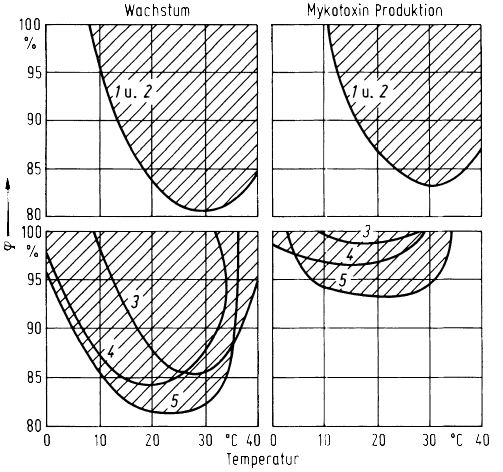
\includegraphics[width=\columnwidth]{misc/awtemp}
}
\item Wie kann die Sicherheit von Lebensmitteln gefährdet werden? Nennen Sie Beispiele. Wie kann die
Sicherheit von Lebensmitteln gewährleistet werden? Wie kann das Wachstum von Mikroorganismen
beeinflusst bzw. kontrolliert werden? Was ist dabei zu beachten?
\antwort{
Die Sicherheit von Lebensmitteln kann durch alle Faktoren aus Frage 9 gefährdet werden. 
Präventive Maßnahmen:
\begin{itemize}
	\item HACCP-Konzept
	\item Temperaturkontrollen
	\item Richtige Lagerung der Lebensmittel (licht, a$_W$, luft)
	\item Bei der Verarbeitung handwerklich gut Arbeiten (Herstellung stabiler Emulsionen, Ausreichende Erhitzung, schnelles Gefrieren, langsames Auftauen)
\end{itemize}
}

\item Wozu verpackt man Lebensmittel? Nennen Sie Beispiele für die Barrierefunktion von Verpackungen
und erläutern Sie die damit verbundenen Prozesse sowie die Schutzeffekte für das Lebensmittel.
Welche Packstoffe können für die Gestaltung von Lebensmittelverpackungen gewählt werden? Wie
unterscheiden sich die unterschiedlichen Packstoffe hinsichtlich ihrer Eigenschaften, und welche
Konsequenzen hat dies für den Einsatz als Lebensmittelverpackung?
\antwort{
\textbf{Gründe:}
\begin{itemize}
	\item Schutz vor mechanischer Beschädigung
	\item Barrierefunktion (Wasser, Wasserdampf, Luft, Gase, etc.)
	\item Abführung von Wärme und Wasser durch Glucoseveratmung
\end{itemize}
\textbf{Packstoffe:}
\begin{itemize}
	\item \textbf{Naturstoffe} wie Holzkisten, Netze, etc.
	\item \textbf{Keramik/Glas} Sehr gute Barriere gegen Gase, Wasser, Aromen, und Chemikalien; bruchempfindlich, schwer; sehr gut zur Langzeitlagerung (z.B. Einmachen)
	\item \textbf{Papier, Pappe} Geringe Barriere gegenüber Feuchtigkeit/Gasen, oft kombiniert mit Kunststoffen oder Metallfolien; umweltfreundlich, leicht
	\item \textbf{Metalle} Fast komplette Barriere gegen Gase, Wasser, Licht (z.B. Konserven); Gefahr von Korrosion (außer wenn innenbeschichtet); schwer, aber robust
	\item \textbf{Kunststoffe} Große Bandbreite an Eigenschaften (z.B. Polyethylen, PET, PA, PVC); können je nach Typ spezifisch als Barriere für Wasser, Sauerstoff, Aromen ausgelegt werden; leicht, formbar, aber teils durchlässiger für Gase und Aromen als Glas oder Metall; Recyclingfähigkeit/Nachhaltigkeit hängt vom Typ ab
\end{itemize}


}
\end{enumerate}

\end{multicols}

%\pagebreak
%\newgeometry{top=2cm,bottom=2cm,left=2cm,right=2cm}
%\section{Formelsammlung}
%\begin{minipage}[t]{.35\textwidth}%
%\large



\textbf{Flüssigkeiten \& Gase}\par \vspace*{-4mm}
%\begin{spacing}{1.5}
\begin{align*}
&\text{Druck:} ~ p = \frac{F}{A} \\
&\text{Kontinuitätsgleichung:} ~ A_1 \cdot v_1 = A_2 \cdot v_2 \\
&\text{Bernoulli:} 		~ p + \rho g h + \frac{1}{2} \rho v^2 = \text{const.} \\[-4pt]
&\quad \text{Staudruck (nach Bernoulli):} ~ p = \frac{1}{2} \rho v^2 \\[-4pt]
&\quad \text{Druck in Wassersäule:} ~ p = \rho gh \\
&\text{Toricelli (Ausfließgeschw.)}: ~ v = \sqrt{2gh} \\[-2pt]
&\qquad t = \sqrt{\frac{2}{g}} \cdot \frac{A_1}{A_2} \cdot (\sqrt{h_{\alpha}}-\sqrt{h_{\omega}})
\end{align*}

\vspace*{8mm}
\textbf{Strömung mit Reibung}\par \vspace*{-4mm}
\begin{align*}
&\text{Volumenstrom:}	~ \dot{V} = \frac{V}{t} = A \cdot \overline{v}\\
&\text{Schubspannung:}	~ \tau = \eta \cdot \frac{d v}{d z} = \frac{F_{R}}{A} \\
&\text{Viskosität:}	~ \eta = \frac{\tau}{D} \\
&\text{Hagen - Poiseuille:} ~ \dot{V} = \frac{\pi R^4}{8\eta} \cdot \frac{d p}{d x}\\
&\text{Leistung} ~ P = \frac{8\eta \cdot \Delta l}{\pi \cdot R^4} \cdot \dot{V}^2\\
&\text{mittlere}\\[-10pt] &\text{Strömungsgeschwindigk.:} ~  c = \overline{v} = \frac{1}{2} \cdot v_{max}
\\ \\
&\text{Stokes'sches Gesetz:} ~ F_r = 6 \pi \eta v r \\[-4pt]
&\quad \text{Stat. Sinkgeschwindigk.:} ~ v = \frac{2r^2g(\rho_1-\rho_2)}{9\eta} \\ \\
&\text{Gesamtwiderstand:} ~ F_{tot} = F_r + F_w\\[-4pt]
&\quad \text{Reibungswiderstand:}  ~ F_r = \eta \cdot A \cdot \frac{d v}{d z}\\[-2pt]
&\quad \text{Widerstandskraft:}  ~ F_w = c_w \cdot A \cdot \frac{1}{2} \rho v^2 \\
\\ 
\end{align*}
\textbf{Rheologie }\par 
\begin{tikzpicture}
\node(a)at(0,0){
\begin{tikzpicture}
\node[align=center,scale=0.8](1)at(0.5,1.5){Newtonsch};
\draw (0,1)node[right]{$\tau$} -- (0,0) -- (1,0)node[right,scale=0.8]{$D$};
\draw[yshift=-1.5cm] (0,1)node[right]{$\eta$} -- (0,0) -- (1,0)node[right,scale=0.8]{$D$};
\draw[black!80] (0,0) -- (0.9,0.9);
\draw[black!80,yshift=-1.5cm] (0,0.5) -- (0.9,0.5);
\end{tikzpicture}
};
\node(b)at(2,0){
\begin{tikzpicture}
\node[align=center,scale=0.8](1)at(0.5,1.5){Scherverdünnend};
\draw (0,1)node[right]{$\tau$} -- (0,0) -- (1,0)node[right,scale=0.8]{$D$};
\draw[yshift=-1.5cm] (0,1)node[right]{$\eta$} -- (0,0) -- (1,0)node[right,scale=0.8]{$D$};
\draw[black!80] (0,0) to [bend left=30] (0.9,0.9);
\draw[black!80,yshift=-1.5cm] (0,0.9) to [bend right=45] (0.9,0.3);
\end{tikzpicture}
};
\node(c)at(4.5,0){
\begin{tikzpicture}
\node[align=center,scale=0.8](1)at(0.5,1.5){Scherverdickend};
\draw (0,1)node[right]{$\tau$} -- (0,0) -- (1,0)node[right,scale=0.8]{$D$};
\draw[yshift=-1.5cm] (0,1)node[right]{$\eta$} -- (0,0) -- (1,0)node[right,scale=0.8]{$D$};
\draw[black!80] (0,0) to [bend right=30] (0.9,0.9);
\draw[black!80,yshift=-1.5cm] (0,0.3) to [bend right=30] (0.9,0.9);
\end{tikzpicture}
};
\node[scale=0.7,rotate=90](fl)at(-1,0.55){Fließkurve};
\node[scale=0.7,rotate=90,align=left](vi)at(-1,-1){Viskositäts-\\kurve};
\end{tikzpicture}
%\end{spacing}
\vfill
\end{minipage}%
%\hspace*{2mm}
%\color{gray!40}
%\vrule
%\color{black}
\hfill
\begin{minipage}[t]{.35\textwidth}
%\large

\textbf{Einheiten \& Konstanten}\par \vspace*{-4mm}

\begin{align*}
%\text{Joule [J]} ~ 	= \frac{\kg \cdot \m^2}{\s^2} \\ %AUSGEBLENDET
&\text{Newton [N]} ~	= \frac{\kg \cdot \m}{\s^2} \\
&\text{Pascal [Pa]} ~	= \frac{\kg}{\m \cdot \s^2} = \ddfrac{\text{N}}{\m^2} \\ 
&\text{Viskosität [$\eta$]} ~	= \text{Pa}\cdot \s = \frac{\text{N} \cdot \s}{\m^2} \\ 
&\text{Watt [W]} ~ = \frac{\kg \cdot \m^2}{\s^3} = \frac{J}{s}\\ \\
&\text{Kritische Reynoldszahl:} \quad \text{Re}_{\text{krit}} = \frac{\rho d v}{\eta} = 2300 \\[-4pt] 
&\text{Stefan-Boltzmann Konst.:} ~\sigma = 5,67 \cdot 10^{-8}~ \text{W}/ \text{m}^{2}\text{K}^{4}\\[1pt]
&\text{Strahlungszahl schw. Körper:} ~C_S = 5,67~ \text{W}/ \text{m}^{2}\text{K}^{4}\\
&\text{Erdbeschleunigung:} \quad g = 9,81 ~\text{m/s}^2 \\[-1pt]
&\text{Dichte von Wasser:} \quad 1000 ~\text{kg/m}^3 \\[-4pt]
&\text{Universelle Gaskonstante: } \quad R = 8,314 \frac{J}{K \cdot mol}
\end{align*}


\vspace*{2mm}
\textbf{Rohre \& Pumpen:}\par \vspace*{-4mm}
\begin{align*}
&\text{Stokes im Rohr:} ~ v = \frac{\Delta p}{4\eta \cdot l \eta} \cdot (R^2-r^2) \\ 
& \hspace*{3cm} v_{max} = \frac{\Delta p \cdot R^2}{4\eta \cdot l \eta} = 2 \cdot \overline{v} \\
&\text{Turbulente Strömungsgeschwindigkeit:}\\ & \quad v = v_{max} \cdot (1-\frac{r}{R})^{1/7}\\[-8pt]
&\hspace*{0.8cm} \scriptstyle{v_{max} \approx 1,2 \cdot \overline{v}}\\
&\text{Volumenstrom:} \quad \dot{V} = \frac{\pi \cdot \Delta p \cdot R^4}{8 \cdot l \cdot \eta} = A_{quer} \cdot \overline{v} \\ 
& \text{Druckabfall im Rohr:} ~ \Delta p = \xi \cdot \frac{l}{d} \cdot \frac{1}{2}\rho\overline{v}^2\\
&\text{Rohrreibungszahl Xi:} ~ \xi_{lam} = \frac{64}{\text{Re}}\\
&\text{Hydraulischer Durchmesser:} ~ d_h = 4\cdot \frac{A}{U}\\
&\text{Nutzleistung Pumpe:} ~ P = \dot{V} \cdot \Delta p_{ges}  \\
\end{align*}




\vspace*{4mm}
\textbf{Strahlung} \par \vspace*{-4mm}
\begin{align*}
&\text{Schwarzkörperstrahlung:} \quad P = \varepsilon \cdot \sigma \cdot A \cdot T^4 \\[-6pt]
&\quad \text{Vereinfacht:} \hspace*{2cm} \quad P = \varepsilon \cdot C_S \cdot A \cdot (\frac{T}{100})^4 \\
&\text{Elektromagn. Strahlung:} \quad E = h \cdot c \cdot \ell^{-1} = h \cdot f \\
&\text{Plank'sches Gesetz:} \quad i = \frac{C_1}{\ell^5 \cdot [\text{exp}(C_2/\ell \cdot T)-1]}
\end{align*}
\end{minipage}%
\vfill
	
	
\pagebreak
\raggedbottom

\begin{minipage}[t]{.45\textwidth}
\vspace*{5.5mm}
\textbf{Wärmelehre} \par \vspace*{-4mm}
\begin{align*}
&\text{Wärmeenergie:} \quad Q = c_m \cdot m \cdot \Delta T \\
&\text{Wärmestromdichte:} \quad \dot{q} = \frac{\dot{Q}}{A} \\
&\text{Konvektion:} \quad \dot{Q} = \alpha \cdot A \cdot \Delta T \\[6pt] 
&\text{Wärmeleitung nach Fourier:}\\
&\quad \text{1.Gesetz:} \quad \dot{Q} = \lambda \cdot A \cdot \frac{\Delta T}{x} \\
&\quad \text{2.Gesetz:} \quad \frac{dT}{dt} = \frac{\lambda}{\rho \cdot c_p} \cdot \frac{d^2T}{dx^2} = a \cdot \frac{d^2T}{dx^2} \\ \\
&\text{Abschätzung Wärmeleitfähigkeit von LM:}\\[4pt]
& \hspace*{2cm} \lambda = \sum \lambda_i \cdot X_Vi \\ \\
&\text{Stat. Wärmeleitung d. Wand mit i Schichten:}\\[4pt]
&\hspace*{2cm} \dot{Q} = \frac{A \cdot \Delta T_{ges}}{\sum \frac{l_i}{\lambda_i}} = \frac{A \cdot \Delta T_{ges}}{R_{ges}}\\ \\
&\text{Stat. Wärmeleitung d. Rohr mit n Schichten:}\\[4pt]
&\hspace*{2cm} \dot{Q} = \frac{2 \pi \cdot l \cdot \Delta T }{\sum \frac{\ln(\frac{r_{a_n}}{r_{i_n}})}{\lambda_n}} \\ \\
&\text{Fläche einer Rohrwand:}\\[4pt]
& \hspace*{2cm} \overline{A} = \frac{A_a - A_i}{\ln(\frac{A_a}{A_i})} = \frac{2 \pi \cdot l \cdot (r_a - r_i)}{\ln(\frac{A_a}{A_i})} \\
\end{align*}


\vspace*{4mm}
\textbf{Kennzahlen turbulente Strömung:} \par \vspace*{-4mm}
\begin{align*}
&\text{Reynoldszahl:} \quad Re = \frac{v \cdot l \cdot \rho}{\eta} = \frac{v \cdot l}{\color{red}{\nu}}
\\
&\text{Grashofzahl:} \quad Gr = - \frac{g \cdot l^3}{{\color{red}{\nu}}^2} \cdot \frac{\Delta p}{p} \\
&\text{Nusseltzahl:} \quad Nu = \frac{\alpha \cdot l}{\lambda} \\
&\text{Prandtlzahl:} \quad Pr = \frac{{\color{red}{\nu}}}{a} = \frac{\eta \cdot c_p}{\lambda} \\ \\
\end{align*}
\par \vspace*{-8mm}
{\color{red} \textit{Kinematische Viskosität $\nu$ in Rot dargestellt.}}
%\par \vspace*{2mm}
%Hier fehlen noch die Formeln für die Beziehung zwischen Nu,Re und Pr für turbulente Strömung im Rohr und Festbett mit runden Partikeln
\end{minipage}\hspace*{8mm}
\begin{minipage}[t]{.35\textwidth}
\vspace*{5.5mm}
\textbf{Diffusion, Packstoffe} \par \vspace*{-4mm}
\begin{align*}
&\text{Säurekonstante:} \quad K_S = \frac{[H^+] \cdot [A^-]}{[HA]} \\ 
&\text{Fick'sches Gesetz:} \quad \dot{n} = D \cdot A \cdot \frac{\Delta c}{l} \\[5pt]
&\text{Henry Gesetz:} \quad c_i = \alpha \cdot p_i \\[3pt]
&\text{Permeation:} \quad J = P \cdot A \cdot \frac{\Delta p}{l}   
\end{align*}
\vspace*{2mm}



\textbf{Dampfdruck, Siedepunkt} \par \vspace*{-4mm}
\begin{align*}
&\text{Clausius-Clapeyron:} \quad \ln(\frac{p_2}{p_1}) = \frac{\Delta h_{vM}}{R} \cdot \left(\frac{1}{T_1} - \frac{1}{T_2} \right) \\
&\text{Siedepunkterhöhung durch gelöste Stoffe:}\\[4pt]
& \Delta T \approx \frac{R \cdot T_L^2}{\Delta h_{vM}} \cdot x_i = \frac{R \cdot T_L^2}{M_L \cdot \Delta h_v} \cdot x_i =\frac{R \cdot T_L^2}{\rho_L \cdot \Delta h_v} \cdot c_i \\
&\text{Siedepunkterhöhung durch hydrostatischen Druck:}\\[4pt]
&\hspace*{2cm} \Delta T = \frac{\rho_{lg} \cdot g \cdot h \cdot R \cdot T_L^2}{\Delta h_{vM} \cdot p}\\
&\text{Siedepunkterhöhung durch Oberflächenspannung:}\\[4pt]
&\hspace*{2cm} \Delta T = \frac{4 \sigma \cdot R \cdot T_L^2}{d \cdot \Delta h_{vM} \cdot p} \\
&\text{Für kontinuierliche Verdampfung benötigter Wärmestrom:}\\[4pt]
&\hspace*{2cm} \dot{Q} = \dot{m}_F \cdot c_{pF} \cdot (T_S - T_F) + \dot{m}_D \cdot \Delta h_v
\end{align*}


\vspace*{2mm}
\textbf{Pasteurisieren, Haltbarmachen} \par \vspace*{-4mm}
\begin{align*}
&\text{Arrhenius-Gleichung:} \quad k = A \cdot e^{-\frac{E_A}{R \cdot T}} \\
&\text{Q$_{10}$-Wert:} \quad Q_{10} = \frac{k_{T+10}}{k_T} \\
&\text{z-Wert:} \quad z = T_{10k} - T_k \\
&\text{Kinetik 1.Ordnung:} \quad \frac{dN}{dt} = -k \cdot N \\
& \hspace*{3.3cm} N(t) = N_0 \cdot e^{-kt} \\
&\text{Dezimalreduktionszeit:} \quad D_1 = D_2 \cdot 10^{\frac{T_2 - T_1}{z}} \\[2pt]
&\hspace*{3.3cm} D = \frac{t_2-t_1}{\log(\frac{N_{(t_1)}}{N_{(t_2)}})} \\
&\text{F-Wert:} \quad F_1 = F_2 \cdot 10^{\frac{T_2 - T_1}{z}} \\
&\text{Inaktivierungsszeit:} \quad F_T = \log(\frac{N_0}{N}) \cdot D_T \\
&\text{Risiko für Kontamination:} \quad \frac{1}{n} = \frac{N_0}{10^{\frac{F}{D}}} 
\end{align*}
\end{minipage}
\end{document}
